% CVPR 2022 Paper Template
% based on the CVPR template provided by Ming-Ming Cheng (https://github.com/MCG-NKU/CVPR_Template)
% modified and extended by Stefan Roth (stefan.roth@NOSPAMtu-darmstadt.de)

\documentclass[10pt,twocolumn,letterpaper]{article}

%%%%%%%%% PAPER TYPE  - PLEASE UPDATE FOR FINAL VERSION
\usepackage{cvpr}      % To produce the REVIEW version
%\usepackage{cvpr}              % To produce the CAMERA-READY version
%\usepackage[pagenumbers]{cvpr} % To force page numbers, e.g. for an arXiv version

% Include other packages here, before hyperref.
\usepackage{graphicx}
\usepackage{amsmath}
\usepackage{amssymb}
\usepackage{booktabs}
\usepackage{tabularx}
\usepackage{multirow}
\usepackage{makecell}
\usepackage{ulem}

% It is strongly recommended to use hyperref, especially for the review version.
% hyperref with option pagebackref eases the reviewers' job.
% Please disable hyperref *only* if you encounter grave issues, e.g. with the
% file validation for the camera-ready version.
%
% If you comment hyperref and then uncomment it, you should delete
% ReviewTempalte.aux before re-running LaTeX.
% (Or just hit 'q' on the first LaTeX run, let it finish, and you
%  should be clear).
\usepackage[pagebackref,breaklinks,colorlinks]{hyperref}


% Support for easy cross-referencing
\usepackage[capitalize]{cleveref}
\crefname{section}{Sec.}{Secs.}
\Crefname{section}{Section}{Sections}
\Crefname{table}{Table}{Tables}
\crefname{table}{Tab.}{Tabs.}


%%%%%%%%% PAPER ID  - PLEASE UPDATE
\def\cvprPaperID{11345} % *** Enter the CVPR Paper ID here
\def\confName{CVPR}
\def\confYear{2025}
\begin{document}

%%%%%%%%% TITLE - PLEASE UPDATE
\title{Hallo3: Highly Dynamic and Realistic Portrait Image Animation with Diffusion Transformer Networks}

\author{Jiahao Cui\textsuperscript{1},
        Hui Li\textsuperscript{1},
        Yun Zhan\textsuperscript{1},
        Hanlin Shang\textsuperscript{1},
        Kaihui Cheng\textsuperscript{1},
        Yuqi Ma\textsuperscript{1},
        Shan Mu\textsuperscript{1},
        Hang Zhou\textsuperscript{2},\\
        Jingdong Wang\textsuperscript{2},\;\;\;
        Siyu Zhu\textsuperscript{1,3} \\
\textsuperscript{1}Fudan University, \;\;\textsuperscript{2}Baidu Inc,
\;\;\textsuperscript{3}Shanghai Academy of AI for Science
 \\
% {\tt\small xxx@xxx}
% For a paper whose authors are all at the same institution,
% omit the following lines up until the closing ``}''.
% Additional authors and addresses can be added with ``\and'',
% just like the second author.
% To save space, use either the email address or home page, not both
}
\maketitle

%%%%%%%%% ABSTRACT
\begin{abstract}
Existing methodologies for animating portrait images face significant challenges, particularly in handling non-frontal perspectives, rendering dynamic objects around the portrait, and generating immersive, realistic backgrounds.
In this paper, we introduce the first application of a pretrained transformer-based video generative model that demonstrates strong generalization capabilities and generates highly dynamic, realistic videos for portrait animation, effectively addressing these challenges.
The adoption of a new video backbone model makes previous U-Net-based methods for identity maintenance, audio conditioning, and video extrapolation inapplicable. To address this limitation, we design an identity reference network consisting of a causal 3D VAE combined with a stacked series of transformer layers, ensuring consistent facial identity across video sequences.
Additionally, we investigate various speech audio conditioning and motion frame mechanisms to enable the generation of continuous video driven by speech audio. Our method is validated through experiments on benchmark and newly proposed wild datasets, demonstrating substantial improvements over prior methods in generating realistic portraits characterized by diverse orientations within dynamic and immersive scenes. Further visualizations and the source code are available at: \href{https://fudan-generative-vision.github.io/hallo3/#/}{https://fudan-generative-vision.github.io/hallo3}.

\end{abstract}

%%%%%%%%% BODY TEXT
\begin{figure*}
    \centering
    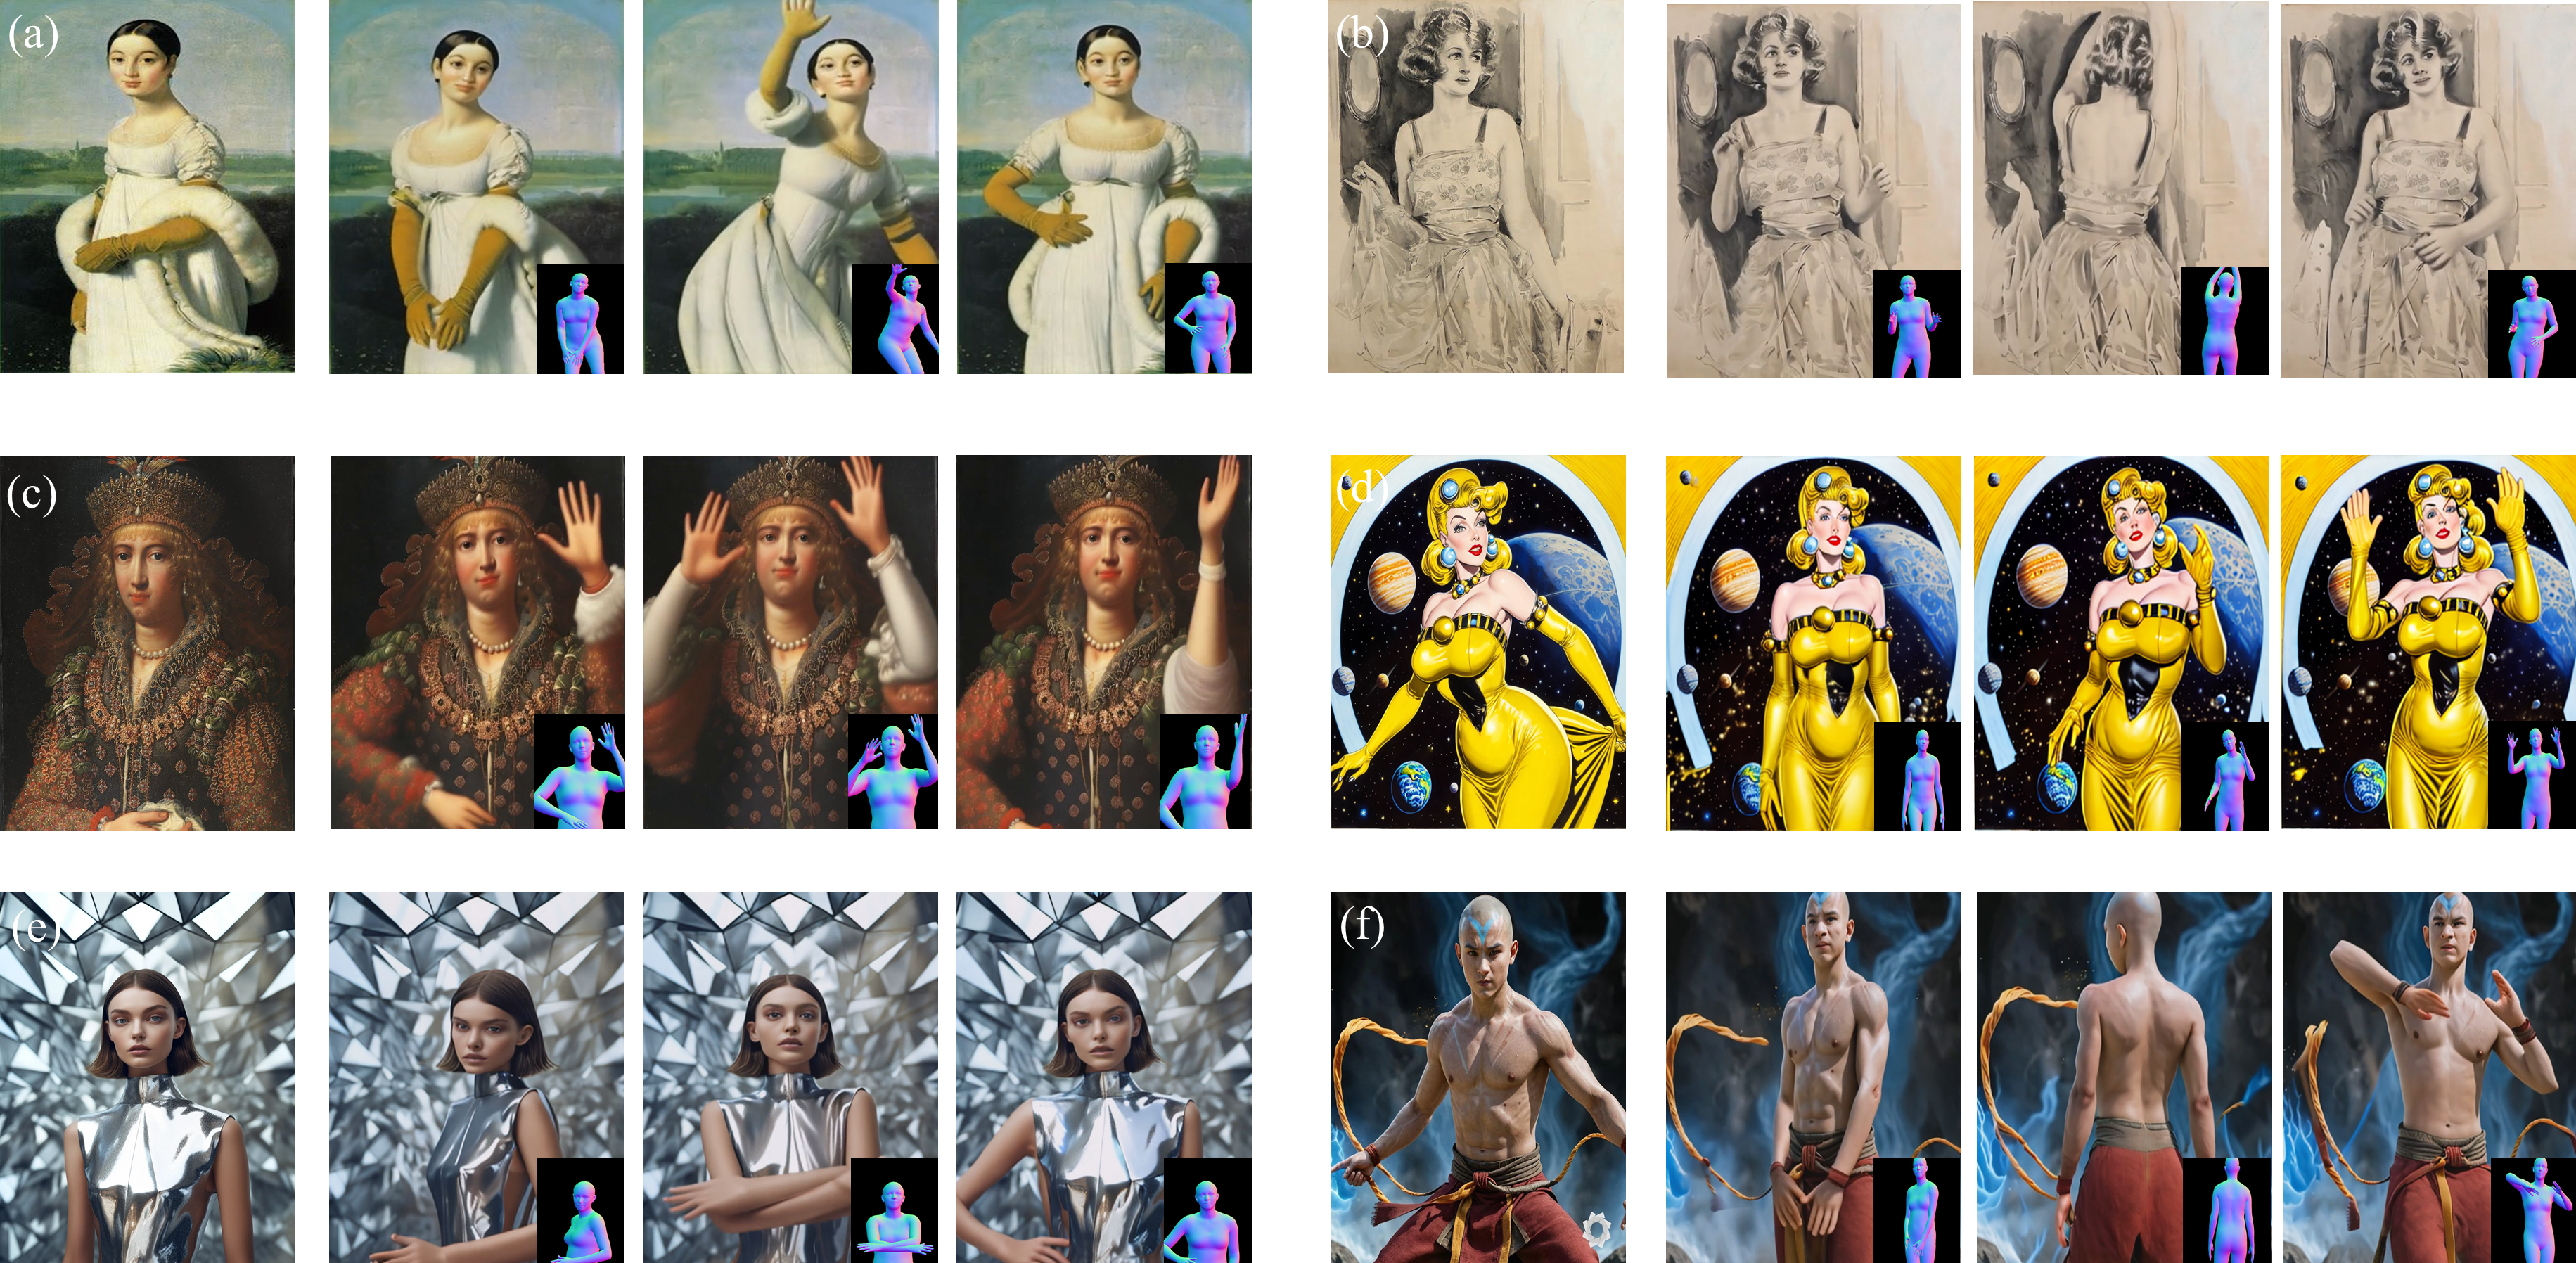
\includegraphics[width=1\linewidth]{figs/teaser.jpg}
    \caption{Demonstration of the proposed approach. Given a reference image, an audio sequence, and a textual prompt, the method generates animated portraits from frontal or different perspectives while preserving the portrait identity over extended durations. Additionally, it incorporates dynamic foreground and background elements, with temporal consistency and high visual fidelity. }
    \label{fig:enter-label}
    \vspace{-5mm}
\end{figure*}

\section{Introduction}
Portrait image animation refers to the process of generating realistic facial expressions, lip movements, and head poses based on portrait images. 
This technique leverages various motion signals, including audio, textual prompts, facial keypoints, and dense motion flow. 
As a cross-disciplinary research task within the realms of computer vision and computer graphics, this area has garnered increasing attention from both academic and industrial communities. 
Furthermore, portrait image animation has critical applications across several sectors, including film and animation production, game development, social media content creation, and online education and training.

In recent years, the field of portrait image animation has witnessed rapid advancements. 
Early methodologies predominantly employed facial landmarks—key points~\cite{siarohin2019first,zakharov2020fast,zhang2022sadtalker} on the face utilized for the localization and representation of critical regions such as the mouth, eyes, eyebrows, nose, and jawline. 
Additionally, these methods~\cite{gao2023high,ren2021pirenderer,zhang2023metaportrait,champ2024} incorporated 3D parametric models, notably the 3D Morphable Model (3DMM)~\cite{blanz2003face}, which captures variability in human faces through a statistical shape model integrated with a texture model. 
However, the application of explicit approaches grounded in intermediate facial representations is constrained by the accuracy of expression and head pose reconstruction, as well as the richness and precision of the resultant expressions.
Simultaneously, significant advancements in Generative Adversarial Networks (GANs) and diffusion models have notably benefited portrait image animation. 
These advancements~\cite{corona2024vlogger,liu2024anitalker,tian2024emo,wei2024aniportrait,xu2024vasa,zhang2024tora,champ2024} enhance the high-resolution and high-quality generation of realistic facial details, facilitate generalized character animation, and enable long-term identity preservation. 
Recent contributions to the field—including Live Portrait~\cite{guo2024liveportrait}, which leverages GAN technology for portrait animation with stitching and retargeting control, as well as various end-to-end methods such as VASA-1~\cite{xu2024vasa}, EMO~\cite{tian2024emo}, and Hallo~\cite{xu2024hallo,cui2024hallo2} employing diffusion models—exemplify these advancements.

Despite these improvements, existing methodologies encounter substantial limitations. 
First, many current facial animation techniques emphasize eye gaze, lip synchronization, and head posture while often depending on reference portrait images that present a frontal, centered view of the subject. 
This reliance presents challenges in handling profile, overhead, or low-angle perspectives for portrait animation. Secondly, accounting for significant accessories, such as holding a smartphone, microphone, or wearing closely fitted objects, presents challenges in generating realistic motion for the associated objects within video sequences.
Third, existing methods often assume static backgrounds, undermining their ability to generate authentic video effects in dynamic scenarios, such as those with campfires in the foreground or crowded street scenes in the background.

Recent advancements in diffusion transformer~(DiT)-based video generation models~\cite{yang2024cogvideox, polyak2024movie, bao2024vidu, liu2024sora} have addressed several challenges associated with traditional video generation techniques, including issues of realism, dynamic movement, and subject generalization. 
In this paper, we present the first application of a pretrained DiT-based video generative model to the task of portrait image animation.
The introduction of this new video backbone model renders previous U-Net-based methods for identity maintenance, audio conditioning, and video extrapolation impractical. 
We tackle these issues from three distinct perspectives.
(1)~\textbf{Identity preservation}: We employ a 3D VAE in conjunction with a stack of transformer layers as an identity reference network, enabling the embedding and injection of identity information into the denoising latent codes for self-attention. This facilitates accurate representation and long-term preservation of the facial subject's identity.
(2)~\textbf{Speech audio conditioning}: We achieve high alignment between speech audio—serving as motion control information—and facial expression dynamics during training, which allows for precise control during inference. We investigate the use of adaptive layer normalization and cross-attention strategies, effectively integrating audio embeddings through the latter.
(3)~\textbf{Video extrapolation}: Addressing the limitations of the DiT-based model in generating continuous videos, which is constrained to a maximum of several tens of frames, we propose a strategy for long-duration video extrapolation. 
This approach uses motion frames as conditional information, wherein the final frames of each generated video serve as inputs for subsequent clip generation.

We validate our approach using benchmark datasets, including HTDF and Celeb-V, demonstrating results comparable to previous methods that are constrained to limited datasets characterized by frontal, centered faces, static backgrounds, and defined expressions. 
Furthermore, our method successfully generates dynamic foregrounds and backgrounds, accommodating complex poses, such as profile views or interactions involving devices like smartphones and microphones, yielding realistic and smoothly animated motion, thereby addressing challenges that previous methodologies have struggled to resolve effectively. 
\section{Related Work}
\label{sec:related_work}

\paragraph{Attention variants and distributed attention}
Ever since attention became popular with the Transformer
architecture~\citep{vaswani2017attention}, there has been a large body of work
on approximating attention to scale it to longer sequences.
These approximation methods can generally be categorized into two classes:
sparse and low-rank.
Sparse attention only computes some entries of the attention matrix ($\mathrm{softmax}(\vQ
\vK^T)$) and assumes that other entries are zero.
Different methods have different ways of choosing which entries should be zero,
either with a fixed pattern~\citep{child2019generating}, with a sliding
window~\citep{beltagy2020longformer}, or with a dynamic pattern through
hashing~\citep{kitaev2020reformer} or routing~\citep{roy2020efficient}.
The low-rank approach instead assumes that the attention matrix has a low-rank
structure, and apply a pointwise nonlinearity to the query and
key~\citep{katharopoulos2020transformers} with random
projection~\citep{choromanski2021rethinking, peng2021random, xiong2021nystromformer}.
One can also combine the sparse and low-rank approximation for better
quality~\citep{zaheer2020bigbird,scatterbrain}.
However, these approximation methods typically do not offer the same model
quality as standard attention~\citep{tay2020efficient}, and so most large-scale
models do not employ these techniques.

There are other variants of attention aimed at reducing the size of the KV cache
to improve inference efficiency. Multi-query attention~\citep{shazeer2019fast} and grouped query
attention~\citep{ainslie2023gqa} tie different heads of $\vK$ and $\vV$, and
multiple query heads interact with the same key and value head.
Multi-head latent attention~\citep{deepseekv2} parameterizes the $\vK$ and $\vV$
as low-rank projections of a shared matrix to further reduce the KV cache size.
However, all of these approaches do not change the core computation
$\mathrm{softmax}(\vQ \vK^T) \vV$ during training and simply change how $\vQ, \vK, \vV$ are
obtained.
As a result, any efficiency or accuracy improvement to the standard attention
computation benefits these methods.

To extend to even longer context, attention computation can be distributed
across multiple GPUs.
Methods such as Ring attention~\citep{liu2023ring,liu2024world} and
variants~\citep{brandon2023striped} can reach a context length of up to 1
million.
They use \fa (or \faa) as a primitive, and so the improvement from \fat would
benefit these distributed attention methods as well.

\paragraph{Alternative architectures}
Motivated by the limitations of attention, a variety of alternative
architectures have been proposed.
They build on the connection between linear
attention~\citep{katharopoulos2020transformers} and recurrent neural networks
(RNNs).
RWKV~\citep{peng2023rwkv}, H3~\citep{dao2023hungry}, MEGA~\citep{ma2023mega},
Retnet~\citep{sun2023retentive}  enhance the expressivity of the simple
cumulative sum in linear attention with more sophisticated recurrences.
Mamba~\citep{gu2023mamba} and xLSTM~\citep{beck2024xlstm} use learnable
weighting for the recurrence and can match the quality of Transformers in
language modeling at small or medium scale.
These approaches can be connected to generalizations of linear attention through
the lens of the structure of the token-mixing matrix~\citep{dao2024transformers}.
These models have started to see some traction, seeing usage in some medium to
large-scale models such as Jamba~\citep{jamba}, Zamba~\citep{zamba},
Megalodon~\citep{ma2024megalodon}, and Mamba2-hybrid~\citep{waleffe2024empirical}.
For the highest quality, these SSM- and RNN-based models still employ
many layers of attention.
We expect that techniques to speed up attention presented in this work will be
useful to speedup these alternative architectures.

\paragraph{Low-precision attention}
Quantization is a promising approach to speed up attention, but they have mostly
focused on reducing the space for KV cache for inference efficiency.
QuIP~\citep{chee2024quip} and QuIP\#\citep{tseng2024quip} use incoherent processing to reduce the quantization,
and we adapted this technique for FP8 \fat.
Recent work suggests that for inference the KV cache is highly compressible down to 4-, 3-, or
even 2-bits~\citep{hooper2024kvquant, liu2024kivi}.
However, quantization during training is still challenging as higher precision
is typically required for stable training.

\paragraph{Hardware-aware Algorithms}
Our work presented in this paper focuses on the micro-architecture
specific tuning to leverage new instruction sets and adopt a natively
asynchronous programming model. There are other orthogonal axes for
hardware-aware algorithm co-design being explored.
A recent example of this is LeanAttention~\citep{sanovar2024-leanattention},
which recognizes the poor GPU occupancy and high memory bandwidth requirements
of the sequential token generation phase as primary bottlenecks for inference
and optimizes it via a smarter load balancing strategy similar to Stream-K
load balancing~\citep{streamk} to achieve nearly peak occupancy.
There is a large literature on optimizing GEMM for specific hardware that employs
many of the same techniques.
As an example, \citet{abdel2016batched} presents a high performance batched GEMM kernel on
K40c Graphics Processing Units (GPU) for both fixed and variable sizes,
proposing specialized GEMM designs
and a comprehensive autotuning process to deliver state-of-the-art 
performance.


%\section{Preliminary}\label{sec:preliminary}
Large language models (LLMs), pretrained on vast corpora, have demonstrated superior capabilities in context understanding and logical reasoning. 
These models have achieved remarkable success across a wide range of tasks in various domains, including natural language processing~\cite{DBLP:journals/corr/abs-2307-06435, DBLP:journals/csur/MinRSVNSAHR24,xu2024large} 
and 
computer vision~\cite{DBLP:conf/nips/LiuLWL23a,DBLP:journals/pami/ZhangHJL24,DBLP:journals/corr/abs-2306-16410}.
Mainstream LLMs, such as GPT~\cite{bubeck2023sparks}, LLaMA~\cite{DBLP:journals/corr/abs-2302-13971}, and DeepSeek~\cite{DBLP:conf/acl/DaiDZXGCLZYWXLH24}, 
are primarily built on the transformer architecture~\cite{vaswani2017attention}. 
To explore the role of Key-Value (KV) cache management in accelerating LLM computations,
we first outline the core components of the transformer model and then introduce the mechanisms for managing the KV cache
to accelerate the LLMs.
Important notations in this survey are summarized in Tab.~\ref{tab:notation}.




\subsection{Transformer Architecture}\label{ssec:transformer}
Transformers~\cite{vaswani2017attention} have become the backbone of LLMs due to their ability to efficiently capture long-range dependencies sequential data, such as text.
This capability makes them particularly well-suited for tasks like machine translation, text generation, and image captioning.
The transformer architecture follows an encoder-decoder structure, where most LLMs utilize only the decoder component.
We first introduce the core components of the Transformer decoder and then describe the critical auto-regressive generation mechanism. 
Particularly, we do not describe certain components in transformer, such as normalization, as they do not impact the understanding of KV cache management.

\begin{table}[t]
    \centering
    \caption{Notation Summary}
    \label{tab:notation}
    \begin{tabular}{c|l}
        \toprule
        \textbf{Symbol} & \textbf{Definition} \\
        \midrule
        $X$ & Input sequence of tokens \\ \hline
        
        $\mathbf{X}$ & Dense representations of  $X$ \\ \hline

        $d_x$ & Dimensionality of the input embeddings. \\\hline

        
        $\mathbf{E}$ & Embedding matrix $\mathbf{E} \in \mathbb{R}^{d_{\text{vocab}} \times d_x}$. \\ \hline
        
        $PE(X)$ & Positional encoding \\ \hline
        
        $\mathbf{Q}_i, \mathbf{K}_i, \mathbf{V}_i$ & Query, Key, and Value matrices \\  \hline

         $d_k, d_v$ & Query/Key and Value dimension \\\hline

        $\mathbf{W}_{Q_i}, \mathbf{W}_{K_i}, \mathbf{W}_{V_i}$ & Weight matrices for computing $\mathbf{Q}_i, \mathbf{K}_i, \mathbf{V}_i$. \\\hline
        
        $\mathbf{Z}_i$ &  Self-attention Output  \\\hline
        
        $\mathbf{W}_O$ & Weight matrix \\\hline
        
        $\mathbf{W}_1, \mathbf{W}_2$ & Weight matrices \\ \hline
        
        $\mathbf{b}_1, \mathbf{b}_2$ & Bias vectors \\\hline
        
      %  $d_o$ & Dimensionality of the concatenated output of multiple attention heads. \\
       % $d_1, d_2$ & Dimensionality of intermediate and output layers in the Feed Forward Network (FFN). \\
       
        $t$ &  Sequence length index \\\hline
        
        $t_c$ & Number of tokens stored in the KV cache. \\ \hline
        
        $\mathbf{K}_i^t, \mathbf{V}_i^t$ & Key and Value at step $t$ \\ \hline        
        $\mathbf{\hat{K}}_i^{t-1}, \mathbf{\hat{V}}_i^{t-1}$ & Cached Key and Value \\\hline
        
        $h$ & Number of attention heads per layer \\\hline
        
        
        $L$ & Number of transformer layers \\\hline
        
      %  $\mathbf{h}_t$ & Hidden state of the LLM at decoding step $t$. \\
        
       % $\mathbf{W}_{\text{out}}, \mathbf{b}_{\text{out}}$ & Output projection matrix and bias vector for predicting the next token. \\
        
        $P(x_{t+1} | x_1, \cdots, x_t)$ & Conditional probability \\
       % $\text{Softmax}$ & Softmax function used to compute attention weights or output probabilities. \\
        \bottomrule
    \end{tabular}
\end{table}

\subsubsection{Transformer Decoder}\label{ssec:decoder}
As shown in Figure~\ref{fig:transformer}, a decoder-based transformer architecture is composed of multiple stacked Transformer blocks, each designed to process sequential data effectively. 
Typically, a Transformer block consists of two core components, i.e., a Multi-Head Self-Attention (MHSA) mechanism and a Feed Forward Network (FFN). 
These blocks are arranged sequentially, where the output of one block is passed as input to the next. This iterative design allows the model to refine its understanding of the input sequence progressively, making it highly effective for tasks such as text generation and language modeling.


\noindent \textbf{Positional Encoding.}
Before the input sequence is processed by the Transformer blocks, it undergoes a preprocessing phase. 
First, a tokenizer processes the input sentence $X$ by splitting it into discrete units, such as words or subwords. The resulting sequence can be represented as 
${X} = [x_1, x_2, \cdots, x_{|X|}]$.
These tokens are then mapped to dense vector representations using an embedding layer, i.e., $\mathbf{X} = \mathbf{I}_X  \mathbf{E}^{\top}$,
where $\mathbf{I}_{X} \in \{0,1\}^{n \times d_{\text{vocab}}}$ represents the one-hot vector of tokenized input $X$, $\mathbf{E} \in \mathbb{R}^{d_{\text{vocab}} \times d_x}$ is the embedding matrix, 
and $\mathbf{X}=[\mathbf{x}_1, \mathbf{x}_2, \cdots, \mathbf{x}_{|X|}]\in \mathbb{R}^{n \times d_{x}}$ is the resulting matrix of embedded token representations.
Since the Transformer architecture does not inherently account for the order of tokens in a sequence, \textbf{positional encodings} are added to the token embeddings $\mathbf{X}$ to incorporate positional information. This can be expressed as $\mathbf{X}=\mathbf{X}+ PE(X)$,
where $PE(X) \in \mathbb{R}^{n \times d_x}$ represents a function~\cite{zhao2023length,zheng2021rethinking,su2024roformer} (e.g., sine and cosine-based positional encoding) that generates positional embeddings for the input ${X}$.


\noindent \textbf{Transformer Block.}
Once the input features are prepared, they are passed through a series of stacked Transformer blocks. Each block begins with the Multi-Head Self-Attention (MHSA) mechanism, which captures both local and global dependencies. For each token, the self-attention mechanism computes a weighted sum over all other tokens in the sequence, where the weights are derived from the similarity between the tokens.
Particularly, since the operations within each transformer block are identical, we use a single transformer block as an example.
Specifically, given the input to a block, denoted as $\mathbf{X} \in \mathbb{R}^{|X| \times d}$, the MHSA mechanism computes the query vectors $\mathbf{Q}_i \in \mathbb{R}^{|X| \times d_k}$, key vectors $\mathbf{K}_i \in \mathbb{R}^{|X| \times d_k}$, and value vectors $\mathbf{V}_i \in \mathbb{R}^{|X| \times d_v}$. These vectors are obtained through learned linear transformations as follows:
\begin{align}\label{eq:qkv}
\mathbf{Q}_i = \mathbf{X}\mathbf{W}_{Q_i}, \quad
\mathbf{K}_i = \mathbf{X}\mathbf{W}_{K_i}, \quad
\mathbf{V}_i = \mathbf{X}\mathbf{W}_{V_i},
\end{align}
where $\mathbf{W}_{Q_i}\in \mathbb{R}^{d_x \times d_k}$, $\mathbf{W}_{K_i} \in \mathbb{R}^{d_x \times d_k}$
and $\mathbf{W}_{V_i} \in \mathbb{R}^{d_x \times d_v}$ are the learned weight parameters.
Then, the self-attention operation is applied to each triple $(\mathbf{Q}_i, \mathbf{K}_i, \mathbf{V}_i)$, and obtain  the output of the $i$-th attention head $\mathbf{Z}_i$ as follows:
\begin{equation}\label{eq:self_attention}
\mathbf{Z}_i = \text{Attention}(\mathbf{Q}_i, \mathbf{K}_i, \mathbf{V}_i) = \text{Softmax}\left(\frac{\mathbf{Q}_i \mathbf{K}_i^\top}{\sqrt{d_k}}\right) \mathbf{V}_i,
\end{equation}
where  $\sqrt{d_k}$  is a scaling factor to ensure the numerical stability. To capture diverse relationships, multiple attention with $h$ heads are applied to $\mathbf{X}$ in parallel, and their outputs are concatenated with one transformation as follows:
\begin{align}\label{eq:self_attention_concat}
\mathbf{Z}=\text{Concat}(\mathbf{Z}_1, \mathbf{Z}_2, \dots, \mathbf{Z}_h)\mathbf{W}_O,
\end{align}
where \text{Concat} is concatenation operation and $\mathbf{W}_O \in \mathbb{R}^{d_v \times d_o}$ is the trainable parameters.




Following the self-attention mechanism, 
the output is passed through a \textbf{Feed Forward Network (FFN)}. The FFN is a fully connected neural network that applies two linear transformations separated by a nonlinear activation function $\sigma(\cdot)$ (e.g, ReLU~\cite{agarap2018deep}) :
\begin{align}\label{eq:ffn}
    \text{FFN}(\mathbf{Z}) = \sigma(\mathbf{Z}\mathbf{W}_1 + \mathbf{b}_1)\mathbf{W}_2 + \mathbf{b}_2
\end{align}
where $\mathbf{W}_1 \in \mathbb{R}^{d_o \times d_1}$ and $\mathbf{W}_2 \in \mathbb{R}^{d_1 \times d_2}$ are  two  parameters.
Also, $\mathbf{b}_1 \in \mathbb{R}^{d_1}$ and $\mathbf{b}_2 \in \mathbb{R}^{d_2}$ are two bias vectors.

\subsubsection{Auto-regressive Generation Mechanism}\label{ssec:auto_regressive}
LLMs employ an autoregressive mechanism to generate text token by token, with each token conditioned on the previously generated ones. This iterative process ensures that the output sequence remains coherent and contextually appropriate.
Formally, given an input sequence of tokens $X = [x_1, x_2, \cdots, x_t]$, 
the model predicts the next token $x_{t+1}$ at each decoding step $t$ by modeling the conditional probability distribution as follows:
\begin{equation}
P(x_{t+1} | x_1, x_2, \cdots, x_t) = \text{Softmax}(\mathbf{h}_t \mathbf{W}_{\text{out}} + \mathbf{b}_{\text{out}}),
\end{equation}
where $\mathbf{h}_t \in \mathbb{R}^{d_h}$ represents the hidden state of the LLM regarding $X$ at step $t$, $\mathbf{W}_{\text{out}} \in \mathbb{R}^{d_h \times vocab}$ is the output projection matrix, and $\mathbf{b}_{\text{out}}$ is the bias vector. 
The softmax function converts the logits into a probability distribution over the vocabulary.
Then,
at each decoding step, the model generates the next token $x_{t+1}$ by sampling from the predicted probability distribution:
\begin{equation}
x_{t+1} \sim P(x_{t+1} | x_1, x_2, \cdots, x_t).
\end{equation}
The generated token $x_{t+1}$ is then appended to the sequence $X=[x_1,\cdots,x_t,x_{t+1}]$, and the process continues until a special end-of-sequence (EOS) token is generated or a predefined maximum length is reached.



 \begin{figure}[t]
    \centering
    \includegraphics[width=0.88\linewidth]{figures/transfomer.pdf}
    \caption{The decoder-only Transformer for LLMs.}
    \label{fig:transformer}
\end{figure}


 


 

\subsection{Key-Value Cache in Transformer Models}\label{ssec:kv_cache}
Auto-regressive generation is a powerful mechanism that enables LLMs to produce high-quality, contextually coherent text. 
However, it presents computational challenges for long sequences, as the Keys and Values need to be recomputed for each token during the generation process. The KV cache optimization addresses this issue by storing the previously computed Keys and Values and reusing them for subsequent token generation, thereby reducing redundant computations and improving inference efficiency.


\subsubsection{Auto-regressive Generation with KV Cache}
Here, we describe how caching KV pairs of tokens accelerates LLM inference. Specifically, at each decoding step \( t \), the model performs self-attention over the entire sequence \( X = [x_1, \cdots, x_{t-1}, x_t] \) to generate the next token \( x_{t+1} \). This process requires the computation of Keys and Values matrices for all previously processed tokens in \( X = [x_1, \cdots, x_t] \).
Notably, when generating the token \( x_t \), the LLM has already computed the Keys and Values for the tokens in \( X[1:t-1] = [x_1, \cdots, x_{t-1}] \). The KV cache optimizes this process by storing the previously computed Keys and Values  matrices for \( X[1:t-1] \) and reusing them, thereby only requiring the computation of Keys and Values for the new token \( x_t \). This significantly improves efficiency by eliminating redundant computations.

Formally, at decoding step $t$, the new token embedding $\mathbf{x}_t$ is used to compute the query vector $\mathbf{q}^t_i$, key vector $\mathbf{k}^t_i$, and value vector $\mathbf{v}^t_i$ as follows:
\begin{align}
\mathbf{q}_i^t &= \mathbf{x}_t \mathbf{W}_{Q_i}, \quad
\mathbf{k}_i^t  = \mathbf{x}_t \mathbf{W}_{K_i}, \quad
\mathbf{v}_i^t  = \mathbf{x}_t \mathbf{W}_{V_i},
\end{align}
The newly computed $\mathbf{k}_i^t $ and $\mathbf{v}_i^t $ are then appended to the cached key and value matrices from previous steps:
\begin{align}
\mathbf{K}_i^{t} &= \text{Concat}(\mathbf{\hat{K}}_i^{t-1}, \mathbf{k}_i^t ), \ 
\mathbf{V}_i^{t} = \text{Concat}(\mathbf{\hat{V}}^{t-1}_i, \mathbf{V}_i^t ),
\end{align}
where $\mathbf{\hat{K}}_i^{t-1} \in \mathbb{R}^{t-1 \times d_k}$ and $\mathbf{\hat{V}}_i^{t-1} \in \mathbb{R}^{t-1 \times d_v}$ represent the cached key and value matrices of tokens in $X[1:t-1]$. 
These cached matrices are then used in the scaled dot-product attention computation for token $x_t$.
%which avoids re-computing attention for previously processed tokens. 
The attention output $\mathbf{z}^t_i$ for the token $x_t$ at step $t$ is calculated as:
\begin{align}
\mathbf{z}^t_i = \text{Softmax}\left(\frac{\mathbf{q}_i^t {\mathbf{K}_i^t}^\top}{\sqrt{d_k}}\right) \mathbf{V}_i^t,
\end{align}
\noindent Then, a similar KV reuse process can be applied to different attention heads in each layer of the LLM.


 
 

\subsubsection{Time and Space Complexity Analysis}\label{sssec:time_space}
Given a transformer-based $L$-layer LLM with $h$ attention heads per layer and an input sequence of length $X = [x_1, \cdots, x_t]$, we analyze the time saved and the space required to store cached KV pairs. For simplicity, we assume the Keys and Values of $t_c$ tokens are stored for all heads across all LLM layers.

\noindent \underline{\textbf{Saved Time.}} 
    For each token,
    the saved computation time comes from avoiding the repeated computation of Keys and Values in Equation~\eqref{eq:qkv}, self-attention result in Equation~\eqref{eq:self_attention}, 
    and linear transformation  in  Equation~\eqref{eq:self_attention_concat}.
     We omit the time analyze on operations in transformer that do not affect  the understanding of KV cache acceleration, such as layer norm and position encoding.

    %and non-linear transformation  in  Equation~\eqref{eq:self_attention_concat} and~\eqref{eq:ffn}.
\begin{itemize}[leftmargin=10pt]
    \item \textbf{QKV Computation.} 
    The time of computing Queries, Keys and Values for each token in Equation~\eqref{eq:qkv} is $\triangle_1 = O(2d_xd_k + d_xd_v)$.
  
    \item  \textbf{Self-attention Result.} 
    Additionally, computing each attention result $\mathbf{z}_i$ in Equation~\eqref{eq:self_attention} takes $O(t(d_k + d_v))$.
    %where $t$ is the sequence length. 

   \item \textbf{Linear Transformation.}
    To merge the $h$ attention results in  Equation~\eqref{eq:self_attention_concat} 
    %and compute the forward result in Equation~\eqref{eq:ffn}, 
    the time is $\triangle_2 = O(hd_v+d_vd_o)$. 

\end{itemize}
Therefore, for $t_c$ cached tokens across $h$ attention heads and $L$ layers, the total saved computation time is:
\begin{align}
    %O\left(L\cdot h \cdot t_c \cdot t \cdot (d_k+d_v)+ L\cdot h \cdot t_c\cdot \triangle_1 \right)
    O\left(L\cdot h \cdot t_c \cdot t \cdot (d_k+d_v)+ L\cdot h \cdot t_c\left(\triangle_1 + \triangle_2\right)\right)
\end{align}
\noindent Thus, the saved time is directly proportional to the number of cached tokens $t_c$, 
significantly accelerating model computation, especially for longer sequences (when $t$ is large).



\noindent \underline{\textbf{Extra Space.}}
Compared to computation without caching, additional space is required to store the cached KV pairs for $t_c$ tokens across $h$ attention heads and $L$ layers. Assuming each Key and Value is stored in Float16 precision, the total extra space needed can be expressed as:
\begin{align}
    O(L\cdot h \cdot t_c \cdot 2 \cdot sizeof(Float16))    
\end{align}
\noindent 
Thus, for the same LLM model, the extra space required to store the KV pairs primarily depends on the number of cached tokens and the precision of the cached Keys and Values. 
To address this, existing approaches explore various techniques to reduce the extra space consumption, such as caching only the most important Keys and Values or applying quantization techniques to lower the bit precision of the stored Keys and Values.






 


\subsection{Challenges in KV Cache Management}\label{ssec:kv_cache_challenge}
As analyzed in Sec.~\ref{sssec:time_space}, 
reusing cached KV pairs enables the LLM to avoid recomputing past tokens, resulting in significant speedups during inference. However, as sequence lengths grow, the size of the KV cache increases proportionally, placing significant pressure on memory. Consequently, it becomes challenging to manage this cache effectively to accelerate LLM computation without excessive space usage.

\begin{itemize}[leftmargin=10pt]
    \item \textbf{Cache Eviction Policies:} 
    Determining which items to evict when the cache reaches its capacity is a complex problem. Popular policies~\cite{podlipnig2003survey} like Least Recently Used (LRU) or Least Frequently Used (LFU) do not align with LLMs  patterns, leading to suboptimal performance.

    \item \textbf{Memory Management:} 
    The memory required for the KV cache grows linearly with both the sequence length and the number of layers, which can quickly exceed the hardware memory limits, especially for long sequences. Consequently, managing the collaboration between different types of storage hardware (e.g., GPU, CPU, or external memory) becomes a significant challenge.




    
    \item \textbf{Latency Bottlenecks:} Accessing and updating the cache at each decoding step can introduce latency, particularly for hardware with limited memory bandwidth.

    \item \textbf{Compression Trade-offs:} Compressing the KV cache can reduce memory usage but may degrade model performance if key information is lost.

    \item \textbf{Dynamic Workloads:} Handling dynamic and unpredictable workloads, where access patterns and data requirements frequently change, requires adaptive caching strategies that can respond in real time.


    \item \textbf{Distributed Coordination:} In distributed KV caches, maintaining coordination across multiple nodes to ensure consistency, fault tolerance, and efficient resource usage adds significant complexity.

\end{itemize}
% \begin{figure*}[!t]
%     \centering
%     \includegraphics[width=1\linewidth]{figs/Pipeline.png}
%     \caption{The overview of the proposed method. Specifically, the method takes reference images, an audio sequence, and textual prompts as inputs to generate a video output with temporal consistency and high visual fidelity. We leverage the casual 3D VAE, T5, and Wav2Vec models to process the visual, textual, and audio features, respectively. The Identity Reference Network extracts identity features from the input reference images and textual prompts, enabling controllable animation while preserving the subject's appearance. The audio encoder generates motion information for lip synchronization, while the face encoder extracts facial features to maintain consistency in facial expressions. The 3D Full Attention and Audio-Attention Modules combine identity and motion data within a denoising network, producing high-fidelity, temporally consistent, and controllable animated videos.}
%     \label{fig:architecture}
%     \vspace{-4 mm}
% \end{figure*}


\begin{figure*}[t!]
    \centering

    % 左侧大图
    \begin{minipage}[b]{0.65\textwidth} % 左侧宽度占40%
        \centering
        \includegraphics[width=\linewidth]{figs/Pipeline_comp.png} % 替换为你的图片路径
        \caption{The overview of the proposed method. Specifically, the method takes a reference image, an audio sequence, and a textual prompt as inputs to generate a video output with temporal consistency and high visual fidelity. We leverage the casual 3D VAE, T5, and Wav2Vec models to process the visual, textual, and audio features, respectively. The Identity Reference Network extracts identity features from the input reference image and textual prompt, enabling controllable animation while preserving the subject's appearance. The audio encoder generates motion information for lip synchronization, while the face encoder extracts facial features to maintain consistency in facial expressions. The 3D Full Attention and Audio-Attention Modules combine identity and motion data within a denoising network, producing high-fidelity, temporally consistent, and controllable animated videos.}
        \label{fig:architecture}

    \end{minipage}
    \hfill
    % 右侧上下两张小图
    \begin{minipage}[b]{0.32\textwidth} % 右侧宽度占55%
        \centering
        \begin{minipage}[b]{\textwidth} % 上方图
                \centering
                \begin{subfigure}{0.3\linewidth} % 增加 subfigure 的宽度
                    \centering
                    \includegraphics[width=\linewidth]{figs/AudioCondition/Audio_SA.png} 
                    \caption{}  
                    \label{fig:AudioConditionSA}  
                \end{subfigure}%
                \hfill
                \begin{subfigure}{0.3\linewidth} % 增加 subfigure 的宽度
                    \centering
                    \includegraphics[width=\linewidth]{figs/AudioCondition/Audio_Ada.png}  
                    \caption{}  
                    \label{fig:AudioConditionAda}  
                \end{subfigure}%
                \hfill
                \begin{subfigure}{0.3\linewidth} % 增加 subfigure 的宽度
                    \centering
                    \includegraphics[width=\linewidth]{figs/AudioCondition/Audio_CA.png}  
                    \caption{}  
                    \label{fig:AudioConditionCA}  
                \end{subfigure}%
                \vspace{-1mm}
                \caption{Different strategies of audio conditioning. (a) self-attention; (b) adaptive norm; (c) cross-attention.}
                \label{fig:AudioCondition}
        \end{minipage}
        % \vspace{0.5cm} % 上下图片间距
        \begin{minipage}[b]{\textwidth} % 下方图
            \centering
            \begin{subfigure}{0.22\linewidth} % 增加 subfigure 的宽度
                \centering
                \includegraphics[width=0.95\linewidth]{figs/RefCondition/FE_CA.png} 
                \caption{}  
                \label{fig:RefConditionCA}  
            \end{subfigure}%
            \hfill
            \begin{subfigure}{0.22\linewidth} % 增加 subfigure 的宽度
                \centering
                \includegraphics[width=0.95\linewidth]{figs/RefCondition/FE_Ada.png}  
                \caption{}  
                \label{fig:RefConditionAda}  
            \end{subfigure}%
            \hfill
            \begin{subfigure}{0.23\linewidth} % 增加 subfigure 的宽度
                \centering
                \includegraphics[width=0.95\linewidth]{figs/RefCondition/VAE_SA.png}  
                \caption{}  
                \label{fig:RefConditionVAESA}  
            \end{subfigure}%
            \hfill
            \begin{subfigure}{0.30\linewidth} % 增加 subfigure 的宽度
                \centering
                \includegraphics[width=\linewidth]{figs/RefCondition/VAE_CA.png}  
                \caption{}  
                \label{fig:RefConditionVAECA}  
            \end{subfigure}%
             \label{fig:RefCondition}
             \vspace{-1mm}
            \caption{{Different strategies of identity conditioning. FE refers to the face encoder. cross-attention demonstrates the best performance. (a) face attention; (b) face adaptive norm; (c) identity reference network; (d) face attention and identity reference network.}}
            \label{fig:IdCondition}
        \end{minipage}
    \end{minipage}
    % \vspace{5mm}
\end{figure*}


 
\section{Methodology}  
This methodology section systematically outlines the approaches employed in our study. 
Section~\ref{sec:baseline} describes the baseline transformer diffusion network, detailing its architecture and functionality. 
Section~\ref{sec:audio} focuses on the integration of speech audio conditions via a cross-attention mechanism. 
Section~\ref{sec:identity} discusses the implementation of the identity reference network, which is crucial for preserving facial identity coherence throughout extended video sequences. 
Section~\ref{sec:train} reviews the training and inference procedures used for the transformer diffusion network. 
Finally, Section~\ref{sec:data} details the comprehensive strategies for data sourcing and preprocessing.

\subsection{Baseline Transformer Diffusion Network}\label{sec:baseline}
\noindent\textbf{Baseline Network.}  
The CogVideoX model~\cite{yang2024cogvideox} serves as the foundational architecture for our transformer diffusion network, employing a 3D VAE for the compression of video data. 
In this framework, latent variables are concatenated and reshaped into a sequential format, denoted as \(\mathbf{z}_t\). 
Concurrently, the model utilizes the T5 architecture~\cite{raffel2023t5} to encode textual inputs into embeddings, represented as \(\mathbf{c}_{\text{text}}\). 
The combined sequences of video latent representations \(\mathbf{z}_t\) and textual embeddings \(\mathbf{c}_{\text{text}}\) are subsequently processed through an expert transformer network. 
To address discrepancies in feature space between text and video, we implement expert adaptive layer normalization techniques, which facilitate the effective utilization of temporal information and ensure robust alignment between visual and semantic data. 
Following this integration, a repair mechanism is applied to restore the original latent variable, after which the output is decoded through the 3D causal VAE decoder to reconstruct the video. 
Furthermore, the incorporation of 3D Rotational Positional Encoding (3D RoPE)~\cite{yang2024cogvideox} enhances the model's capacity to capture inter-frame relationships across the temporal dimension, thereby establishing long-range dependencies within the video framework.  

\noindent\textbf{Conditioning in Diffusion Transformer.}  
In addition to the textual prompt \(\mathbf{c}_{\text{text}}\), we introduce two supplementary conditions: the speech audio condition \(\mathbf{c}_{\text{audio}}\) and the identity appearance condition \(\mathbf{c}_{\text{id}}\).  

Within diffusion transformers, four primary conditioning mechanisms are identified: in-context conditioning, cross-attention, adaptive layer normalization (adaLN), and adaLN-zero~\cite{Peebles2022DiT}. 
Our investigation primarily focuses on cross-attention and adaptive layer normalization (adaLN). Cross-attention enhances the model's focus on conditional information by treating condition embeddings as keys and values, while latent representations serve as queries. 
Although adaLN is effective in simpler conditioning scenarios, it may not be optimal for more complex conditional embeddings that incorporate richer semantic details, such as sequential speech audio. Relevant comparative analyses will be elaborated upon in the experimental section.  

\subsection{Audio-Driven Transformer Diffusion}\label{sec:audio}
\noindent\textbf{Speech Audio Embedding.}  
To extract salient audio features for our proposed model, we utilize the wav2vec framework developed by Schneider et al.~\cite{schneider2019wav2vec}. The audio representation is defined as \(\mathbf{c}_{\text{audio}}\). 
Specifically, we concatenate the audio embeddings generated by the final twelve layers of the wav2vec network, resulting in a comprehensive semantic representation capable of capturing various audio hierarchies. 
This concatenation emphasizes the significance of phonetic elements, such as pronunciation and prosody, which are crucial as driving signals for character generation. 
To transform the audio embeddings obtained from the pretrained model into frame-specific representations, we apply three successive linear transformation layers, mathematically expressed as: $\mathbf{c}_{\text{audio}}^{(f)} = \mathcal{L}_3 \left( \mathcal{L}_2 \left( \mathcal{L}_1 \left( \mathbf{c}_{\text{audio}} \right) \right) \right)$, where \(\mathcal{L}_1\), \(\mathcal{L}_2\), and \(\mathcal{L}_3\) represent the respective linear transformation functions. This systematic approach ensures that the resulting frame-specific representations effectively encapsulate the nuanced audio features essential for the performance of our model.  

% \begin{figure}[th!]
% \vspace{-2mm}
%     \centering
%     \begin{subfigure}{0.3\linewidth} % 增加 subfigure 的宽度
%         \centering
%         \includegraphics[width=\linewidth]{figs/AudioCondition/Audio_SA.png} 
%         \caption{Self-Attention}  
%         \label{fig:AudioConditionSA}  
%     \end{subfigure}%
%     \hfill
%     \begin{subfigure}{0.3\linewidth} % 增加 subfigure 的宽度
%         \centering
%         \includegraphics[width=\linewidth]{figs/AudioCondition/Audio_Ada.png}  
%         \caption{Adaptive Norm}  
%         \label{fig:AudioConditionAda}  
%     \end{subfigure}%
%     \hfill
%     \begin{subfigure}{0.3\linewidth} % 增加 subfigure 的宽度
%         \centering
%         \includegraphics[width=\linewidth]{figs/AudioCondition/Audio_CA.png}  
%         \caption{Cross-Attention}  
%         \label{fig:AudioConditionCA}  
%     \end{subfigure}%
    
%     \caption{Different strategies of audio conditioning. Cross-Attention demonstrates the best performance.}
%     \label{fig:AudioCondition}
%     \vspace{-4mm}
% \end{figure}


\noindent\textbf{Speech Audio Conditioning.}  
We explore three fusion strategies---self-attention, adaptive normalization, and cross-attention---as illustrated in Figure~\ref{fig:AudioCondition} to integrate audio condition into the DiT-based video generation model. Our experiments show that the cross-attention strategy delivers the best performance in our model. For more details, please refer to Section~\ref{sec:ablationstudy}. 

Following this, 
 we integrate audio attention layers after each face-attention layer within the denoising network, employing a cross-attention mechanism that facilitates interaction between the latent encodings and the audio embeddings. 
Specifically, within the DiT block, the motion patches function as keys and values in the cross-attention computation with the hidden states \(\mathbf{z}_t\): $\mathbf{z}_t = \text{CrossAttention}(\mathbf{z}_t, \mathbf{c}_{\text{audio}}^{(f)})$. This methodology leverages the conditional information from the audio embeddings to enhance the coherence and relevance of the generated outputs, ensuring that the model effectively captures the intricacies of the audio signals that drive character generation.  




\subsection{Identity Consistent Transformer Diffusion}\label{sec:identity}

% \begin{figure}[th!]
%     \centering
%     \begin{subfigure}{0.22\linewidth} % 增加 subfigure 的宽度
%         \centering
%         \includegraphics[width=0.95\linewidth]{figs/RefCondition/FE_CA.png} 
%         \caption{}  
%         \label{fig:RefConditionCA}  
%     \end{subfigure}%
%     \hfill
%     \begin{subfigure}{0.22\linewidth} % 增加 subfigure 的宽度
%         \centering
%         \includegraphics[width=0.95\linewidth]{figs/RefCondition/FE_Ada.png}  
%         \caption{}  
%         \label{fig:RefConditionAda}  
%     \end{subfigure}%
%     \hfill
%     \begin{subfigure}{0.23\linewidth} % 增加 subfigure 的宽度
%         \centering
%         \includegraphics[width=0.95\linewidth]{figs/RefCondition/VAE_SA.png}  
%         \caption{}  
%         \label{fig:RefConditionVAESA}  
%     \end{subfigure}%
%     \hfill
%     \begin{subfigure}{0.30\linewidth} % 增加 subfigure 的宽度
%         \centering
%         \includegraphics[width=\linewidth]{figs/RefCondition/VAE_CA.png}  
%         \caption{}  
%         \label{fig:RefConditionVAECA}  
%     \end{subfigure}%
%      \label{fig:RefCondition}
%     \caption{{Different strategies of identity conditioning. FE refers to the face encoder. Cross-Attention demonstrates the best performance. (a) Face attention; (b) Face adaptive norm; (c) Identity reference network; (d) Face attention and Identity reference network.}}

% \end{figure}



\noindent\textbf{Identity Reference Network.}  
Diffusion transformer-based video generation models encounter significant challenges in maintaining facial identity coherence, particularly as the length of the generated video increases. 
While incorporating speech audio embeddings as conditional features can establish a correspondence between audio speech and facial movements, prolonged generation often leads to rapid degradation of facial identity characteristics.  

To address this issue, we introduce a control condition within the existing diffusion transformer architecture to ensure long-term consistency of facial identity appearance. 
{We explore four strategies~(as shown in Figure~\ref{fig:IdCondition}) for appearance conditioning: 1) Face attention, where identity features are encoded by the face encoder and combined with a cross-attention module; 2) Face adaptive norm, which integrates features from the face encoder with an adaptive layer normalization technique; 3) Identity reference network, where identity features are captured by a 3D VAE and combined with some transformer layers; and 4) Face attention and Identity reference network, which encodes identity features using both the face encoder and 3D VAE, combining them with self-attention and cross-attention. Our experiments show that the combination with Face attention and Identity reference net achieves the best performance in our model. For further details, please refer to Section~\ref{sec:ablationstudy}. }

We treat a reference image as a single frame and input it into a causal 3D VAE to obtain latent features, which are then processed through a reference network consisting of 42 transformer layers. Mathematically, if \(\mathbf{I}_{\text{ref}}\) denotes the reference image, the encoder function of the 3D VAE is defined as: $\mathbf{z}_\text{id} = \mathcal{E}_{3D}(\mathbf{I}_{\text{ref}})$,
where \(\mathbf{z}_{\text{id}}\) represents the latent features associated with the reference image.  

During the operation of the reference network, we extract vision tokens from the input of the 3D full attention mechanism for each transformer layer, which serve as reference features \(\mathbf{z}_{\text{id}}\). These features are integrated into corresponding layers of the denoising network to enhance its capability, expressed as: $\mathbf{z}_{t, \text{enhanced}} = \text{SelfAttention}(\mathbf{z}_t, \mathbf{z}_{\text{id}}),$
where \(\mathbf{z}_t\) is the latent representation at time step \(t\). 
Given that both the reference network and denoising network leverage the same causal 3D VAE with identical weights and comprise the same number of transformer layers (42 layers in our implementation), the visual features generated from both networks maintain semantic and scale consistency. 
This consistency allows the reference network's features to incorporate the appearance characteristics of facial identity from the reference image while minimizing disruption to the original feature representations of the denoising network, thereby reinforcing the model's capacity to generate coherent and identity-consistent facial animations across longer video sequences.

\noindent\textbf{Temporal Motion Frames.}  
To facilitate long video inference, we introduce the last \(n\) frames of the previously generated video, referred to as motion frames, as additional conditions. Given a generated video length of \(L\) and the corresponding latent representation of \(l\) frames, we denote the motion frames as \(N\). 
The motion frames are processed through the 3D VAE to obtain \(n\) frames of latent codes. 
We apply zero padding to the subsequent \((l-n)\) frames and concatenate them with \(l\) frames of Gaussian noise. 
This concatenated representation is then patchified to yield vision tokens, which are subsequently input into the denoising network. By repeatedly utilizing motion frames, we achieve temporally consistent long video inference.



\subsection{Training and Inference}\label{sec:train}

\noindent\textbf{Training.}  
%The objective of the training process is to minimize the expected mean squared error between actual and predicted noise, framed by the loss function: $\mathcal{L} = \mathbb{E}_{\mathbf{z}_0, \mathbf{c}, \boldsymbol{\epsilon}, t} \left[ \omega(t) \left\| \boldsymbol{\epsilon} - \boldsymbol{\epsilon}_{\theta}(\mathbf{z}_t, t, \mathbf{c}) \right\|_2^2 \right]$, where \(\omega(t)\) serves as a weighting function to balance the loss in various time steps.  
The training process consists of two phases:

\textbf{(1) Identity Consistency Phase.} In this initial phase, we train the model to generate videos with consistent identity. The parameters of the 3D Variational Autoencoder (VAE) and face image encoder remain fixed, while the parameters of the 3D full attention blocks in both the reference and denoising networks, along with the face attention blocks in the denoising network, are updated during training. The model’s input includes a randomly sampled reference image from the training video, a textual prompt, and the face embedding. The textual prompt is generated using MiniCPM\cite{yao2024minicpm}, which describes human appearance, actions, and detailed environmental background. The face embedding is extracted via InsightFace\cite{insightface2024}. With these inputs, the model generates a video comprising 49 frames.

\textbf{(2) Audio-Driven Video Generation Phase.} In the second phase, we extend the training to include audio-driven video generation. We integrate audio attention modules into each transformer block of the denoising network, while fixing the parameters of other components and updating only those of the audio attention modules. Here, the model's input consists of a reference image, an audio embedding, and a textual prompt, resulting in a sequence of 49 video frames driven by audio.
% \text{}(1) In the first phase, we train the model to output videos with consistency of identity. The parameters of the 3D VAE and face image encoder are fixed, while the parameters of the 3D full attention in the reference network, composed of a series of transformer blocks, and those in the denoising network, including the 3D full attention and face attention, are updated through training. The model's input comprises a randomly sampled reference image from the training video, a textual prompt, and the face embedding obtained from the face encoder, with the output being a sequence of 49 frames of video. 
% (2) In the second phase, we train the model for audio-driven video generation. We insert audio attention modules into each transformer block of the denoising network, fixing the parameters of the other components and updating only those of the audio attention modules. The model's input consists of the reference image, input audio, and textual prompt, yielding a sequence of 49 frames of video.

\noindent\textbf{Inference.}  
%After training, new samples can be generated by initializing from a random Gaussian latent vector \(\mathbf{z}_T \sim \mathcal{N}(\mathbf{0}, \mathbf{I})\) and applying the iterative denoising process, defined as: $\mathbf{z}_{t-1} = \frac{1}{\sqrt{\alpha_t}} \left( \mathbf{z}_t - \frac{1 - \alpha_t}{\sqrt{1 - \bar{\alpha}_t}} \, \boldsymbol{\epsilon}_{\theta}(\mathbf{z}_t, t, \mathbf{c}) \right) + \sigma_t \mathbf{n}$, where \(\mathbf{n} \sim \mathcal{N}(\mathbf{0}, \mathbf{I})\) and \(t\) iterates from \(T\) to \(1\). The original image is reconstructed by decoding the final latent vector \(\mathbf{z}_0\) using the VAE decoder, yielding the generated output image represented as \(\mathbf{I} = \mathcal{D}(\mathbf{z}_0)\).  
During inference, the model receives a reference image, a segment of driving audio, a textual prompt, and motion frames as inputs. 
The model then generates a video that exhibits identity consistency and lip synchronization based on the driving audio. 
To produce long videos, we utilize the last two frames of the preceding video as motion frames, thereby achieving temporally consistent video generation.


% \begin{itemize}
%     \item \textbf{Extraction of Single-Speaker Video Clips:}
%     \begin{itemize}
%         \item \textbf{Shot Splitting and Re-encoding}: We employed scene detection and ffmpeg tools to split the videos into individual shots and re-encode them at a frame rate of 25 fps or lower, ensuring synchronization between audio and video data.
%         \item \textbf{Audio Processing}: Utilizing Ultimate Vocal Remover technology, we eliminated background music and environmental sounds from the videos, retaining only the vocal components. This step was crucial for ensuring alignment between audio embeddings and lip movements in the video.
%         \item \textbf{Segment Extraction}: Through the application of pyannote's speaker diarization and overlapped speech detection tools, we accurately extracted segments featuring a single speaker, ensuring that each video clip contained only one speaker's voice.
%     \end{itemize}

%     \item \textbf{Face and Camera Motion Filter:}
%     \begin{itemize}
%     \item **Facial Displacement Filter:** We employed InsightFace technology to calculate facial displacement in the videos, filtering out data where the facial displacement within a 17-frame window exceeded 50\% of the facial bounding box. This step ensured stable character movements and reduced facial blurriness due to rapid motion.
%     \item **Facial Rotation Filter:** Similarly, we utilized InsightFace technology to compute the facial rotation angles, particularly horizontal yaw, filtering out data with an average horizontal rotation exceeding 40°. This measure ensured that the faces in the videos were generally oriented towards the camera.
%     \item ** Camera Motion Filter:** Using CoTracker technology, we detected camera motion classifications in the videos and filtered out data exhibiting dynamic camera movements to minimize interference from moving backgrounds.
%     \item **Audio Lip Sync Filter:** We employed SyncNet technology to compute the audio-visual synchronization scores of the videos, filtering out data with scores below 5.0.
%     \end{itemize}
%     \item \textbf{Data Post-processing:}
%     \begin{itemize}
%         \item **Video Cropping:** Based on the facial positions detected in the previous steps, we cropped the videos into segments with a 3:2 aspect ratio to meet the model's input requirements.
%         \item **Facial Encoding:** A random frame's face was selected, and InsightFace technology was utilized to encode it into embeddings, providing essential facial feature information for the model.
%         \item **Audio Encoding:** The audio from the videos was extracted and encoded into embeddings using Wav2Vec2 technology, facilitating the injection of audio conditions during model training.
%     \end{itemize}
% \end{itemize}

    % \item \textbf{Facial Displacement Calculation:} We employed insightface technology to calculate facial displacement in the videos, filtering out data where the facial displacement within a 17-frame window exceeded 50\% of the facial bounding box. This step ensured stable character movements and reduced facial blurriness due to rapid motion.
    
    % \item \textbf{Facial Rotation Angle Calculation:} Similarly, we utilized insightface technology to compute the facial rotation angles, particularly horizontal yaw, filtering out data with an average horizontal rotation exceeding 40°. This measure ensured that the faces in the videos were generally oriented towards the camera.
    
    % \item \textbf{Camera Motion Classification Detection:} Using CoTracker technology, we detected camera motion classifications in the videos and filtered out data exhibiting dynamic camera movements to minimize interference from moving backgrounds.
    
    % \item \textbf{SyncNet Score Calculation:} We employed SyncNet technology to compute the audio-visual synchronization scores of the videos, filtering out data with scores below 5.0.


\begin{figure*}[t]
    \centering
    \includegraphics[width=\linewidth]{figs/dataset_comp.png}
    \vspace{-7mm}
    \caption{{
Illustration of the dataset, including the flow of data processing, data distribution across different metric, and the visualization of some representative portrait images for inference.}}
    \label{fig:data_statistics}
    % \vspace{-4mm}
\end{figure*}


\subsection{Dataset}\label{sec:data}



In this section, we will give a detailed introduction of our data curation, including data sources, filtering strategy and data statistics.
Figure~\ref{fig:data_statistics} shows the data pipeline and the statistical analysis of the final data.

\noindent\textbf{Data Sources}
The training data used in this work is prepared from three distinct sources to ensure diversity and generalization. Specifically, the sources are: (1) HDTF dataset~\cite{zhang2021flow}, which contains 8 hours of raw video footage; (2) YouTube data, which consists of 1,200 hours of public raw videos; (3) a large scale movie dataset, which contains film videos of 2,346 hours. 
Our dataset contains a large scale of human identities and, however, we find that YouTube and movie dataset contains  a large amount of noised data. Therefore, we design a data curation pipeline as follows to construct a high-quality and diverse talking dataset, as shown in Figure~\ref{fig:data_statistics}(a).

% \begin{itemize}

%     \item \textbf{HDTF Dataset:} this open-source Talking Face video dataset provides 8 hours of raw video footage. After extensive cleaning and preprocessing, 6 hours of high-quality data are curated for model training.
    
%     \item \textbf{YouTube Data:} We collect 1,200 hours of video data from YouTube, and apply a thorough cleaning process that involved removing duplicates, low-quality videos, and irrelevant content. Finaly, 72 hours of high-quality video are left for training.
    
%     \item \textbf{Film Data:}  To diversify the dataset, we collect and construct a large scale movie video dataset, which contains 2,346 hours. After data curation, 53 hours of video data are retained.
% \end{itemize}



\noindent\textbf{Video Filtering.}
During the data pre-processing phase, we implement a series of meticulous filtering steps to ensure the quality and applicability of the dataset. The workflow includes three stages: extraction of single-speaker, motion filter and post-processing. Firstly, we select video of single-speaker. This stage aims to clean the video content to solve camera shot, background noise, etc, using existing tools~\cite{Plaquet23,Bredin23}. After that, we apply several filtering techniques to ensure the quality of head motion, head pose, camera motion, etc~\cite{karaev23cotracker,karaev24cotracker3,Chung16a}. In this stage, we compute all metric scores for each clip, therefore, we can flexibly adjust data screening strategies to satisfy different data requirement of our multiple training stages or strategies. Finally, based on the facial positions detected in previous steps, we crop the videos to a 3:2 aspect ratio to meet the model's input requirements. We then select a random frame from each video and use InsightFace~\cite{ren2023pbidr} to encode the face into embeddings, providing essential facial feature information for the model. Additionally, we extract the audio from the videos and encode it into embeddings using Wav2Vec2 model~\cite{baevski2020wav2vec}, facilitating the incorporation of audio conditions during model training.

\noindent\textbf{Data Statistics.}
Following the data cleaning and filtering processes, we conducted a detailed analysis of the final dataset to assess its quality and suitability for the intended modeling tasks. Finally, our training data contains about 134 hours of videos, including 6 hours of high-quality data from HDTF dataset, 72 hours of YouTube videos, and 56 hours of movie videos. Figure~\ref{fig:data_statistics}(b) also shows other statistics, such as Lip Sync score~(Sync-C and Sync-D), face rotation, face ratio~(the ratio of face height to video height).
%As can be seen in Fig~\ref{fig:data_statistics}b, our dataset has a large.





\begin{table*}[t!]
    \centering
    % 第一个表格
    \begin{minipage}{0.25\textwidth}
        \centering
        \resizebox{\textwidth}{!}{
        \begin{tabular}{c|c|c|c|c}
        \toprule
        \ &
          \multicolumn{1}{c|}{FID$\downarrow$} &
          \multicolumn{1}{c|}{FVD$\downarrow$} &
          \multicolumn{1}{c|}{Sync-C$\uparrow$} &
          \multicolumn{1}{c}{Sync-D$\downarrow$} \\ 
          \midrule
        SadTalker~\cite{zhang2022sadtalker}   & 22.340 & 203.860 & \textbf{7.885} & \textbf{7.545}  \\
        DreamTalk~\cite{ma2023dreamtalk}      & 78.147 & 790.660 & 6.376 & 8.364  \\
        AniPortrait~\cite{wei2024aniportrait} & 26.561 & 234.666 & 4.015 & 10.548  \\
        Hallo~\cite{xu2024hallo}              & 20.545 & 173.497 & 7.750 & 7.659  \\
        Ours                                  & \textbf{20.359} & \textbf{160.838} & 7.252 & 8.106  \\ 
        \midrule
        Real video                            & - & - & 8.700 & 6.597 \\ 
        \bottomrule
        \end{tabular}}
        \vspace{-2mm}
        \caption{Comparison with the other methods on HDTF dataset.} 
        \label{tab:comp_hdtf}
    \end{minipage}
    \hfill
    % 第二个表格
    \begin{minipage}{0.30\textwidth}
        \centering
        \resizebox{\textwidth}{!}{
        \begin{tabular}{c|c|c|c|c|c}
        \toprule
            \ &
              \multicolumn{1}{c|}{FID$\downarrow$} &
              \multicolumn{1}{c|}{FVD$\downarrow$} &
              \multicolumn{1}{c|}{Sync-C$\uparrow$} &
              \multicolumn{1}{c|}{Sync-D$\downarrow$} &
              \multicolumn{1}{c}{E-FID$\downarrow$} \\ 
              \midrule
            SadTalker~\cite{zhang2022sadtalker}   & 50.015 & 471.163 & 6.922 & \textbf{7.921} & 95.194 \\
            DreamTalk~\cite{ma2023dreamtalk}      & 109.011 & 988.539 & 5.709 & 8.743 & 153.450 \\
            AniPortrait~\cite{wei2024aniportrait} & 46.915 & 477.179 & 2.853 & 11.709 & 88.986 \\
            Hallo~\cite{xu2024hallo}              & 44.578 & 377.117 & \textbf{7.191} & 7.984 & 78.495 \\
            Ours                                  & \textbf{43.271} & \textbf{355.272} & 6.527 & 9.113 & \textbf{71.210} \\ 
            \midrule
            Real video                            & - & - & 7.372 & 7.518 & - \\ 
            \bottomrule
        \end{tabular}}
        \vspace{-2mm}
        \caption{Comparison with other methods on Celeb-V dataset.}
        \label{tab:comp_celebv}
    \end{minipage}
    \hfill
    % 第三个表格
    \begin{minipage}{0.39\textwidth}
        \centering
        \resizebox{\textwidth}{!}{
        \begin{tabular}{c|c|c|c|c|c|c}
        \toprule
        \ &
          \multicolumn{1}{c|}{Sync-C$\uparrow$} &
          \multicolumn{1}{c|}{Sync-D$\downarrow$} &
          \makecell{Subject\\Dynamic$\uparrow$} &
          \makecell{Background\\Dynamic$\uparrow$} &
          \makecell{Subject\\FVD$\downarrow$} &
          \makecell{Background\\FVD$\downarrow$} \\ 
          \midrule   
        SadTalker~\cite{zhang2022sadtalker}  & 3.845           & 10.378         & 2.953   & 0.220 & 470.377 &313.758 \\
        DreamTalk~\cite{ma2023dreamtalk}     & 4.498           & 11.005         & 6.958   & 1.806 & 835.480 &744.177 \\
        AniPortrait~\cite{wei2024aniportrait}&	1.685           & 12.025        & 3.351  & 1.769 & 473.173 & 302.716 \\
        Hallo~\cite{xu2024hallo}             & 4.654           & 10.202         & 5.268   & 1.272 & 394.627 & 291.052 \\
        Ours                                 & \textbf{6.154}  & \textbf{8.574} & 
         \textbf{13.286}  & \textbf{4.481} & \textbf{359.493} &\textbf{248.283} \\ 
        \bottomrule
        \end{tabular}}
        \vspace{-2mm}
        \caption{Comparison with other methods on our proposed wild dataset.}
        \label{tab:comparison_wild}
    \end{minipage}
    \vspace{2mm}
\end{table*}


\begin{figure*}[t!]
    \centering
    \includegraphics[width=\linewidth]{figs/HTDF_CelebV_comp.jpg}
    \vspace{-6mm}
    \caption{Qualitative comparison on the HTDF~(left) and CelebV~(right) data-set.}
    \vspace{-2mm}
    \label{fig:hdtf}
\end{figure*}





% \begin{figure}[th!]
%     \centering
%     % Creates an empty box with dimensions
%     % \rule{\linewidth}{0.5\linewidth}
%     \includegraphics[width=1\linewidth]{figs/comparisn_of_audio_conditioning2.pdf}
%     \caption{Qualitative comparison of different strategies for audio conditioning.}
%     \label{fig:comparisn_of_audio_conditioning2}
%     \vspace{-4mm}
% \end{figure}

% \begin{figure}[th!]
%     \centering
%     % Creates an empty box with dimensions
%     % \rule{\linewidth}{0.5\linewidth}
%      \includegraphics[width=1\linewidth]{figs/Comparison_of_the_appearance_reference_network.pdf}
%     \caption{ Qualitative comparison of different strategies for indentity conditioning.}
%     \label{fig:Comparison_of_the_appearance_reference_network}
% \end{figure}

\section{Experiment}
\subsection{Experimental Setups}
% \noindent\textbf{Comparison on dynamic scene scenarios.}

\noindent\textbf{Implementation.}
% {The model was trained using 64 NVIDIA A100 GPUs. In addition to training, all experiments were conducted on a GPU server equipped with 8 NVIDIA A100 GPUs. The first and second stages of the model were trained 20,000 steps respectively. During training, the batch size of each GPU was 1, and the learning rate was set to 1e-5. The resolution of the training video is 480 x 720, and it can generate a video with 49 frames at a time. In the training process, the audio embedding is dropped with a probability of 0.05, and the motion frames are randomly masked with a probability of 0.25.}
We initialize the identity reference and denoising networks with weights derived from CogVideoX-5B-I2V\cite{yang2024cogvideox}. During both training phases, we employ the v-prediction diffusion loss\cite{salimans2022progressive} for optimization. Each training phase comprises 20,000 steps, utilizing 64 NVIDIA H100 GPUs. The batch size per GPU is set to 1, with a learning rate of \(480 \times 720\) pixels. To enhance video generation variability, the reference image, guidance audio and textual prompt are dropped with a probability of 0.05 during training.

\noindent\textbf{Evaluation Metrics.}
We employed a range of evaluation metrics for generated videos across benchmark datasets, including HDTF~\cite{zhang2021flow} and Celeb-V~\cite{zhu2022celebvhq}. 
These metrics comprise Fréchet Inception Distance (FID)~\cite{Seitzer2020FID}, Fréchet Video Distance (FVD)~\cite{unterthiner2018towards}, Synchronization-C (Sync-C)~\cite{Chung16a}, Synchronization-D (Sync-D)~\cite{Chung16a}, and E-FID~\cite{tian2024emo}. 
FID and FVD quantify the similarity between generated images and real data, while Sync-C and Sync-D assess lip synchronization accuracy. E-FID evaluates the image quality based on features extracted from the Inception network.
Besides, we introduced VBench~\cite{huang2023vbench} metrics to enhance evaluation, focusing on dynamic degree and subject consistency. 
% Background consistency is evaluated via CLIP feature similarity, assessing the temporal stability of backgrounds. 
%Temporal flickering is quantified by mean absolute differences in static frames, while motion smoothness is analyzed using motion priors from a video frame interpolation model. 
Dynamic degree is measured using RAFT~\cite{teed2020raft} to quantify the extent of motion in generated videos, providing a comprehensive assessment of temporal quality.
Subject consistency is measured through DINO~\cite{caron2021emerging} feature similarity, ensuring uniformity of a subject's appearance across frames. 


\noindent\textbf{Baseline Approaches.}
We considered several representative audio-driven talking face generation methods for comparison, all of which have publicly available source code or implementations. These methods include SadTalker~\cite{zhang2022sadtalker}, DreamTalk~\cite{ma2023dreamtalk}, AniPortrait~\cite{wei2024aniportrait}, and Hallo~\cite{xu2024hallo,cui2024hallo2}. 
The selected approaches encompass both GANs and diffusion models, as well as techniques utilizing intermediate facial representations alongside end-to-end frameworks. 
This diversity in methodologies allows for a comprehensive evaluation of the effectiveness of our proposed approach compared to existing solutions.

% Subject consistency is measured through DINO feature similarity, ensuring uniformity of a subject's appearance across frames. 
% Background consistency is evaluated via CLIP feature similarity, assessing the temporal stability of backgrounds. 
%Temporal flickering is quantified by mean absolute differences in static frames, while motion smoothness is analyzed using motion priors from a video frame interpolation model. 
%Dynamic degree is measured using RAFT to quantify the extent of motion in generated videos, providing a comprehensive assessment of temporal quality.

%\noindent\textbf{Datasets} Our dataset comprises HDTF~\cite{zhang2021flow} as well as additional data sourced from the Internet. In order to build a dataset of both high quality and diversity, we have designed a comprehensive data curation pipeline capable of processing a wide variety of Internet videos, including YouTube and movie clips. Specifically, we collected 1200 hours of YouTube videos and 2346 hours of movie footage, from which we curated 128 hours of high-quality video clips. The details of the pipeline and related statistics are presented in Figure~\ref{fig:data_statistics}. For further discussions, please refer to the Appendix.





\subsection{Comparison with State-of-the-art}

\noindent\textbf{Comparison on HDTF and Celeb-V Dataset.}
{As shown in Table~\ref{tab:comp_hdtf} and ~\ref{tab:comp_celebv}, our method achieves best results on FID, FVD on both datasets. Although our approach shows some disparity compared to the state-of-the-art in lip synchronization, it still demonstrates promising results as illustrated in Figure~\ref{fig:hdtf}. This is because, to generate animated portraits from different perspectives, our training data primarily consists of talking videos with significant head and body movements, as well as diverse dynamic scenes, unlike static scenes with minimal motion. While this may lead to some performance degradation on lip synchronization, it better reflects realistic application scenarios. }
%We find that large head pose diversity~(such as large head turning) and head motion may lead to the degeneration. 

%\noindent\textbf{Comparison on Celeb-V Dataset.}
%\textcolor{red}{Table~\ref{tab:comp_celebv} presents quantitative comparison on CelebV dataset. }
% and qualitative 



\noindent\textbf{Comparison on Wild Dataset.} 
To effectively demonstrate the performance of the general talking portrait video generation, we carefully collect 34 representative cases for evaluation. This dataset consists of portrait images with various head proportions, head poses, static and dynamic scenes and complex headwears and clothing. To achieve comprehensive assessment, we evaluate the performance on lip synchronization~(Sync-C and Sync-D), motion strength (subject and background dynamic degree) and  video quality~(subject and background FVD).
As shown in Table~\ref{tab:comparison_wild}, our method generates videos with largest head and background dynamic degree~(13.286 and 4.481) while keeping lip synchronization of highest accuracy. 

Figure~\ref{fig:portrait_complex_face} provides a qualitative comparison of different portrait methods on a ``wild" dataset. The results reveal that other methods struggle to animate side-face portrait images, often resulting in static poses or facial distortions. Additionally, these methods tend to focus solely on animating the face, overlooking interactions with other objects in the foreground---such as the dog next to the elderly, or the dynamic movement of the background---like the ostrich behind the girl. In contrast, as shown in Figure~\ref{fig:ComplexScenes} our method produces realistic portraits with diverse orientations and complex foreground and background scenes.



\begin{figure*}[t!]
    \hspace{-2.5mm}
    \centering    \includegraphics[width=1.01\linewidth]{figs/method_comparison3_2.jpg}
    \vspace{-7mm}
    \caption{Complex facial identity with dynamic accessories subjects and different pose orientation.}
    
    \label{fig:portrait_complex_face}
    \vspace{2mm}
\end{figure*}

\begin{figure*}[t!]
    \centering
    \includegraphics[width=1.0\linewidth]{figs/ComplexScenes.jpg}
    \vspace{-6mm}
    \caption{Complex scenes with dynamic foreground or background and various head poses.}
    \label{fig:ComplexScenes}
    \vspace{-2mm}
\end{figure*}










\subsection{Ablation Study and Discussion}
\label{sec:ablationstudy}
\noindent\textbf{Audio Conditioning.} {Table~\ref{tab:audio_injection} and Figure~\ref{fig:comparisn_of_audio_conditioning2} illustrate the effects of various strategies for incorporating audio conditioning. The results demonstrate that using cross-attention to integrate audio improves lip synchronization by enhancing the local alignment between visual and audio features, particularly around the lips. This is evident from the improvements in Sync-C and Sync-D, and it also contributes to a degree of enhancement in video quality.}

\noindent\textbf{Identity Reference Network.} {
Table~\ref{tab:identity_preserve} and Figure~\ref{fig:Comparison_of_the_appearance_reference_network} evaluate different identity conditioning strategies.  The results indicate that without an identity condition, the model fails to preserve the portrait appearance. When using face embedding alone, the model introduces blur and distortion, as it focuses solely on facial features and disrupts the global visual context. To address this, we introduce an identity reference network to preserve global features while making facial motion more controllable through identity-based facial embeddings. Thus, the proposed method achieves a lower FID of 23.458 and FVD of 242.602, while maintaining lip synchronization.
}

\noindent\textbf{Temporal Motion Frames.} {Table~\ref{tab:motion_frame_num} presents an analysis of varying temporal motion frames. One motion frame achieves the highest Sync-C score (6.889) and the lowest Sync-D score (8.695), indicating substantial lip synchronization.}

% \subsection{Limitations and Future Works}
% \textcolor{red}{This paper presents advancements in wild portrait image animation with different perspective and complex scenes, there exist several limitations that necessitate further exploration and consideration. (1)...}
% \begin{table}[]
% \centering
% \footnotesize
% \begin{tabular}{lc|l|l|l|l|l|l}
% \cline{2-8}
%  &
%   FD & PG &
%   \multicolumn{1}{c|}{FID$\downarrow$} &
%   \multicolumn{1}{c|}{FVD$\downarrow$} &
%   \multicolumn{1}{c|}{Sync-C$\uparrow$} &
%   \multicolumn{1}{c|}{Sync-D$\downarrow$} &
%   \multicolumn{1}{c}{E-FID$\downarrow$} \\ \cline{2-8} 
%  &            &            & - & - & - & - & - \\
%  & \checkmark &            & - & - & - & - & - \\
%  &            & \checkmark & - & - & - & - & - \\
%  & \checkmark & \checkmark & - & - & - & - & - \\ \cline{2-8} 
% \end{tabular}
% \caption{Ablation on augmentation for id preservation. FD: Frame drop; PG: Pixel Gaussian}
% \label{tab:abl_id_augment}
% \end{table}


\noindent
\textbf{CFG Scales for Diffusion Model.}  
Table~\ref{tab:abalation_cfg} provides a quantitative analysis of video generations using various CFG scales for audio, text, and reference images. A comparison between the second and fourth rows demonstrates that increasing the audio CFG scale enhances the model's ability to synchronize lip movements. The text CFG scale significantly influences the video’s dynamism, as indicated in the first three rows, where both the subject's and the background's dynamics increase with higher text CFG scales. Conversely, the reference image CFG scale primarily governs the subject's appearance; higher values improve subject consistency, as illustrated by the second and fifth rows. Among the tested configurations, setting \(\lambda_a=3.5\), \(\lambda_t=3.5\), and \(\lambda_i=1.0\) yields a balanced performance. This interplay between visual fidelity and dynamics underscores the effectiveness of CFG configurations in generating realistic portrait animations.


\begin{figure*}[!t]
    \centering
    \begin{minipage}{0.48\linewidth}
        \centering
        \includegraphics[width=\linewidth]{figs/comparisn_of_audio_conditioning3.pdf}
        \vspace{-7mm}
        \caption{Qualitative comparison of different strategies for audio conditioning.}
        \label{fig:comparisn_of_audio_conditioning2}
        \vspace{16.5mm}
    \end{minipage}
    \hfill% 手动添加间距
    \begin{minipage}{0.48\linewidth}
        \centering
        \includegraphics[width=1\linewidth]{figs/Comparison_of_the_appearance_reference_network2.pdf}
        \vspace{-7mm}
        \caption{Qualitative comparison of different strategies~(as in Table~\ref{tab:identity_preserve}) for identity conditioning. 
        (a) No identity condition; (b) Face attention; (c) Face adaptive norm; (d) Identity reference network; (e) Face attention and Identity reference network. 
        }
        \label{fig:Comparison_of_the_appearance_reference_network}
    \end{minipage}
    \vspace{-3mm}
\end{figure*}




\begin{table}[t!]
\vspace{-16mm}
\centering
\footnotesize
\resizebox{\linewidth}{!}{
\begin{tabular}{c|c|c|c|c}
\toprule
  \makecell{Audio Injection Method} &
  \multicolumn{1}{c|}{FID$\downarrow$} &
  \multicolumn{1}{c|}{FVD$\downarrow$} &
  \multicolumn{1}{c|}{Sync-C$\uparrow$} &
  \multicolumn{1}{c}{Sync-D$\downarrow$} \\ 
  \midrule
 adaLN       & 24.159 & 264.331 & 1.374 & 13.524 \\
 adaLN-zero  & 24.029 & 276.403 & 1.398 & 13.553 \\ 
 Self Attn.  & 24.748 & 270.101 & 1.345 & 13.456 \\
 \midrule
 Cross Attn.~(Ours) & \textbf{23.458} & \textbf{242.602} & \textbf{4.601} & \textbf{10.416} \\
 \bottomrule
\end{tabular}
}
\vspace{-2mm}
\caption{Comparison on the different strategy of audio conditioning.}
\label{tab:audio_injection}
\vspace{-1mm}
\end{table}


\begin{table}[t!]
\centering
\footnotesize
\resizebox{\linewidth}{!}{
\begin{tabular}{c|c|c|c|c|c}
\toprule
  \makecell{Identity Injection Method} &
  \multicolumn{1}{c|}{FID$\downarrow$} &
  \multicolumn{1}{c|}{FVD$\downarrow$} &
  \multicolumn{1}{c|}{Sync-C$\uparrow$} &
  \multicolumn{1}{c|}{Sync-D$\downarrow$} & 
  \multicolumn{1}{c}{ Subject Consistency$\uparrow$} \\ 
  \midrule
 (a) No identity condition & 32.304 & 371.820 & 3.183 & 11.732 & 0.977 \\
 (b) Face attention & 57.541 & 740.536 & 4.042 & 10.682 & 0.974 \\
 (c) Face adaptive norm & 150.720 & 1587.395 & 3.822 & 12.324 & 0.904 \\
 (d) Identity reference network & 28.789 & 291.863 & 4.553 & \textbf{10.317} & 0.984 \\
 \midrule
 (e) Face attention and Identity reference network  & \textbf{23.458} & \textbf{242.602} & \textbf{4.601} & 10.416 & \textbf{0.988} \\ 
 \bottomrule
\end{tabular}
}
\vspace{-2mm}
\caption{Comparison of different identity injection method. ``No identity condition'' refers to the absence of any conditioning related to identity; ``Face attention'' and ``Face adaptive norm'' involve incorporating face embeddings using self-attention and adaptive layer normalization, respectively. ``Identity reference network'' refers to the introduction of identity features using a reference network.}
\label{tab:identity_preserve}
\vspace{-1mm}
\end{table}

\begin{table}[t!]
\centering
\footnotesize
\resizebox{\linewidth}{!}{
\begin{tabular}{c|c|c|c|c}
\toprule
  \makecell{Motion Frame Number} &
  \multicolumn{1}{c|}{FID$\downarrow$} &
  \multicolumn{1}{c|}{FVD$\downarrow$} &
  \multicolumn{1}{c|}{Sync-C$\uparrow$} &
  \multicolumn{1}{c}{Sync-D$\downarrow$} \\ 
  \midrule 
 n = 1     & 24.040 & 242.708 & \textbf{6.889} & \textbf{8.695} \\
 n = 2     & \textbf{23.458} & \textbf{242.602} & 4.601 & 10.416 \\
 n = 4     & 24.459 & 269.904 & 5.109 & 10.489 \\
 n = 8     & 27.303 & 265.396 & 5.114 & 10.464 \\ 
 \bottomrule 
\end{tabular}
}
\vspace{-2mm}
\caption{Ablation on the number of motion frames.}
\label{tab:motion_frame_num}
\vspace{-6mm}
\end{table}

\begin{table*}[th!]
    \centering
    \resizebox{\linewidth}{!}{
    \begin{tabular}{c|ccc|c|c|c|c|c|c|c}
    \toprule
    &Audio & Text & Image & 
    Sync-C$\uparrow$ & Sync-D$\downarrow$ & 
    \makecell{Subject\\Dynamic$\uparrow$} & 
    \makecell{Background\\Dynamic$\uparrow$} & 
    \makecell{Subject\\FVD$\downarrow$} & 
    \makecell{Background\\FVD$\downarrow$} &
    \makecell{Subject\\Consistency$\uparrow$}\\ 
    \midrule
    $\lambda_t \downarrow$ &$\lambda_a = 3.5$ & $\lambda_t=1.0$ & $\lambda_i=1.0$ &  6.168 & 8.589 & 13.164 & \ \ \ 3.955 $\downarrow$ & 361.582 & 263.416 & 0.9813 \\ 
    Base &$\lambda_a=3.5$ & $\lambda_t=3.5$ & $\lambda_i=1.0$ &  6.154 & 8.574 & 13.286 & 4.481 & 359.493 & 248.283 & 0.9810 \\ 
    $\lambda_t \uparrow$ &$\lambda_a=3.5$ & $\lambda_t=6.0$ & $\lambda_i=1.0$ &  6.044 & 8.861 & 13.616 & \ \ \ 4.659 $\uparrow$ & 342.894 & 235.307 & 0.9808 \\ 
    $\lambda_a \uparrow$&$\lambda_a=6.0$ & $\lambda_t=3.5$ & $\lambda_i=1.0$ &  \ \ \ 6.469 $\uparrow$ & 8.515 & 14.778 & 4.066 & 379.073 & 264.969 & 0.9809 \\  
    $\lambda_i \uparrow$&$\lambda_a=3.5$ & $\lambda_t=3.5$ & $\lambda_i=3.5$ & 6.023 & 8.654 & 12.599 & 4.219 & 367.225 & 265.414 & \ \ \ 0.9835 $\uparrow$ \\ 
    \bottomrule
    \end{tabular}}
    \vspace{-3mm}
    \caption{ Quantitative study of audio, text and image CFG scales on our proposed wild dataset. }
    \vspace{-2mm}
    \label{tab:abalation_cfg}
\end{table*}

\noindent\textbf{Limitations and Future Works.}
Despite the advancements in portrait image animation techniques presented in this study, several limitations warrant acknowledgment. 
While the proposed methods improve identity preservation and lip synchronization, the model's ability to realistically represent intricate facial expressions in dynamic environments still requires refinement, especially under varying illumination conditions. 
Future work will focus on enhancing the model's robustness to diverse perspectives and interactions, incorporating more comprehensive datasets that include varied backgrounds and facial accessories. 
Furthermore, investigating the integration of real-time feedback mechanisms could significantly enhance the interactivity and realism of portrait animations, paving the way for broader applications in live media and augmented reality.

\noindent\textbf{Safety Considerations.}
The advancement of portrait image animation technologies, particularly those driven by audio inputs, presents several social risks, most notably concerning the ethical implications associated with the creation of highly realistic portraits that may be misused for deepfake purposes. 
To address these concerns, it is essential to develop comprehensive ethical guidelines and responsible use practices.
Moreover, issues surrounding privacy and consent are prominent when utilizing individuals' images and voices. It is imperative to establish transparent data usage policies, ensuring that individuals provide informed consent and that their privacy rights are fully protected.
By acknowledging these risks and implementing appropriate mitigation strategies, this research aims to promote the responsible and ethical development of portrait image animation technology.

\subsection{Generation Controllability}

\noindent\textbf{Textual Prompt for Subject Animation.}
To evaluate whether textual conditional controllability is effectively preserved, we conducted a series of experiments comparing the performance of our method to that of the baseline model, CogVideoX~\cite{yang2024cogvideox}, using same text prompts. As shown in Figure~\ref{fig:inter}, the results shows that our model maintains its ability for textual control, and effectively captures the interaction between different subjects as dictated by the textual prompts.
% (e.g.,the rabbit, horse and birds.)

\noindent\textbf{Textual Prompt for Foreground and Background Animation.} We also explore model's ability to follow the foreground and background textual prompt. As illustrated in Figure~\ref{fig:fgbg}, our method animates the foreground and background subjects naturally, such as the ocean waves and flickering candlelight. The results demonstrates the model's ability to control foreground, and background with the textual caption, which is maintained even after introducing the audio condition.

\begin{figure*}[!h]
    \centering
    \includegraphics[width=.97\linewidth]{figs/text_cond_interact.pdf}
    \vspace{-4mm}
    \caption{{Condition on interacting with subjects. Our method achieves alignment comparable to that of CogVideX, maintaining the controllability of interactive subjects even after introducing the audio condition.}}
    \vspace{-2mm}
    \label{fig:inter}
\end{figure*}

\begin{figure*}[!h]
    \centering
    \includegraphics[width=.97\linewidth]{figs/text_cond_bgfg.pdf}
    \vspace{-4mm}
    \caption{{Textual condition on foreground and background. Our method achieves alignment comparable to that of CogVideX, maintaining the controllability of foreground and background after incorporating the audio condition. }}
    \label{fig:fgbg}
    \vspace{-3mm}
\end{figure*}


\section{Conclusion}

This paper introduces advancements in portrait image animation utilizing the enhanced capabilities of a transformer-based diffusion model. By integrating audio conditioning through cross-attention mechanisms, our approach effectively captures the intricate relationship between audio signals and facial expressions, achieving substantial lip synchronization. To preserve facial identity across video sequences, we incorporate an identity reference network. Additionally, we utilize motion frames to enable the model to generate long-duration video extrapolations. Our model produces animated portraits from diverse perspectives, seamlessly blending dynamic foreground and background elements while maintaining temporal consistency and high fidelity.



%%%%%%%%% REFERENCES
{\small
\bibliographystyle{ieee_fullname}
\bibliography{egbib}
}
% \section{Appendix} \label{appendix}


\subsection{NewYorker Data for evaluation}

\begin{figure}[!ht]
\small
\centering
\includegraphics[width=0.4\textwidth]{figures/length.png}
\caption{\label{lengthdist} Distribution of word count of stories in our test set}
\end{figure}

Table \ref{teststories} shows the data used for conducting our evaluation. The 12 stories shown are taken from The New Yorker and summarized into single-sentence plots. These stories come from highly established literary experts acting as an upper bound for what it means to be creative. These stories span complex themes.

\begin{table*}[!ht]
\centering
\small
\def\arraystretch{1.35}
\begin{tabular}{|l|}
\hline
\begin{tabular}[c]{@{}l@{}}Write a New Yorker-style story given the plot below. Make sure it is atleast \textbf{\color{blue}\{\{word\_count\}\}} words. Directly start with the\\ story, do not say things like `Here's the story {[}...{]}:\end{tabular}                                                                                                                                                                                            \\ \hline\hline
\begin{tabular}[c]{@{}l@{}}You wrote the story I gave you below. I requested a story with \textbf{\color{blue}\{\{word\_count\}\}} words, but the story only has\\ \textbf{\color{blue}\{\{current\_word\_count\}\}} words. Can you rewrite the story to make it longer, and closer to the \textbf{\color{blue}\{\{word\_count\}\}} word target\\ I gave you. Directly start with the story, do not say things like `Here's the story {[}...{]}:`\\ \\ Current story: \{\{story\}\}\end{tabular} \\ \hline
\end{tabular}
\vspace{2ex}
\caption{\label{promptstory}Prompt to write the initial story (Row1) vs Prompt to rewrite the initial story to be longer. word\_count represents the number of words in the human written story on a given plot (P) while current\_word\_count represents the number of words in the LLM generated story on the same plot (P)}
\end{table*}

\begin{table*}[!ht]
\def\arraystretch{1.15}
\small
\begin{tabular}{|l|l|}
\hline
Story                                    & Plot                                                                                                                                                                                                                                                                                                                                                                                                                                                                                                                                   \\ \hline
\href{https://www.newyorker.com/books/flash-fiction/a-triangle}{A Triangle}                               & \begin{tabular}[c]{@{}l@{}}An observer becomes entranced by a seemingly ordinary couple on the street, follows them home, and then \\watches them from outside in the rising floodwaters, drawing an eerie connection between the woman and\\ a discarded, burned chair they'd noticed earlier.\end{tabular}                                                                                                                                                                    \\ \hline\hline
\href{https://www.newyorker.com/books/flash-fiction/barbara-detroit-1966}{\begin{tabular}[c]{@{}l@{}}Barbara\\ Detroit,1966\end{tabular}}                    & \begin{tabular}[c]{@{}l@{}}On Feb 12, 1966, a heavily pregnant woman named Barbara experienced a shocking incident in her synagogue\\in Southfield, Detroit, where a young man shot and killed the renowned Rabbi Adler before turning the gun\\ on himself, and though Barbara tried to reach the shooter, she was swept away by the fleeing crowd.\end{tabular}                                                                              \\ \hline\hline
\href{https://www.newyorker.com/books/flash-fiction/beyond-nature}{Beyond Nature}                           & \begin{tabular}[c]{@{}l@{}}A solitary man walking in a remote mountainous region comes across a car crash, and stays by the side\\ of the lifeless female victim, narrating stories of his past and reflecting on the impermanence of \\events and life itself, while awaiting emergency services amidst the looming presence of wilderness.\end{tabular}                                                                                                                \\ \hline\hline
\href{https://www.newyorker.com/books/flash-fiction/certain-european-movies}{\begin{tabular}[c]{@{}l@{}}Certain European\\ Movies\end{tabular}}                  & \begin{tabular}[c]{@{}l@{}}Two individuals, at a residency together, navigate the complexity of their ephemeral relationship during\\ their final beach trip, framed by misadventures, subtle tensions, unspoken desires, and looming departures.\end{tabular}                                                                                                                                                                                   \\ \hline\hline
\href{https://www.newyorker.com/books/flash-fiction/keys}{Keys}                                     & \begin{tabular}[c]{@{}l@{}}Daniel, struggling with recurring dreams of his ex-wife Rachel and a mysterious unused flat, eventually \\discusses them with his current partner Isabel, sparking various reflections and conversations about their\\ past relationships, until a real-life discovery of old keys triggers a nostalgic memory and helps him find a\\ way to reconnect with his present relationship through canoeing.\end{tabular}                                     \\ \hline\hline
\href{https://www.newyorker.com/books/flash-fiction/listening-for-the-click}{\begin{tabular}[c]{@{}l@{}}Listening For\\ the Click\end{tabular}}                  & \begin{tabular}[c]{@{}l@{}}Navigating a complex social landscape, the protagonist experiences a series of complex relationships \\and emotional turmoil in a student environment, and engages in self-discovery and self-reflection as she\\ interacts with the characters Carl, Martin, Lizzy, and Johan, resulting in a journey of introspection,\\ betrayal, love, and personal growth.\end{tabular}                                                          \\ \hline\hline
\href{https://www.newyorker.com/magazine/2023/05/15/maintenance-hvidovre-fiction-olga-ravn}{\begin{tabular}[c]{@{}l@{}}Maintenance,\\ Hvidovre\end{tabular}}                   & \begin{tabular}[c]{@{}l@{}}A woman experiences a disorienting night in a maternity ward where she encounters other similarly \\disoriented new mothers, leading to an uncanny mix-up where she leaves the hospital with a baby \\that she realizes is not her own, yet accepts the situation with an inexplicable sense of happiness.\end{tabular}                                                                                                  \\ \hline\hline
\href{https://www.newyorker.com/magazine/2022/11/14/returns}{Returns}                                  & \begin{tabular}[c]{@{}l@{}}The narrator visits their elderly mother in her small town, spending a day with her that is filled with \\nostalgia, conversation, and old habits, only to return a month later after her hospitalization due to\\ a sunstroke, finding remnants of their last visit.\end{tabular}                                                                                                                                                                      \\ \hline\hline
\href{https://www.newyorker.com/books/flash-fiction/the-facade-renovation-thats-going-well}{\begin{tabular}[c]{@{}l@{}}The Facade \\Renovation\\ That’s Going Well\end{tabular}} & \begin{tabular}[c]{@{}l@{}}An academic faculty housed in a building with a critical waterproofing layer missing experiences a series\\ of disruptive and problematic construction repairs, causing tension, inconvenience, and health concerns\\ among the tenants, ultimately leading to resignation and endurance in hopes of better future circumstances.\end{tabular}                                                        \\ \hline\hline
\href{https://www.newyorker.com/books/flash-fiction/the-kingdom-that-failed}{\begin{tabular}[c]{@{}l@{}}The Kingdom\\ That Failed\end{tabular}}                  & \begin{tabular}[c]{@{}l@{}}The narrator recounts their college friendship with the seemingly flawless Q, and after a decade apart, \\they accidentally cross paths at a pool, where the narrator anonymously observes Q's failed attempt to \\let down a woman about a work-related issue, demonstrating that Q, too, has his share of difficulties.\end{tabular}                                                                                                \\ \hline\hline
\href{https://www.newyorker.com/magazine/2022/06/13/trash }{Trash}                                    & \begin{tabular}[c]{@{}l@{}}A woman unexpectedly marries the son of a successful, ambitious woman named Miss Emily, finding both \\acceptance and critique from her mother-in-law as she navigates this new relationship and confronts the \\stark contrasts between her former life as a supermarket cashier and her new life as part of a well-off family.\end{tabular}                                                                                                            \\ \hline\hline
\href{https://www.newyorker.com/culture/personal-history/the-last-dance-with-my-dad}{\begin{tabular}[c]{@{}l@{}}The Last Dance\\ with my Dad \end{tabular}}               & \begin{tabular}[c]{@{}l@{}}A young teenager recounts her experiences of fitting into her father's gay lifestyle, highlighted by a\\ seven-day cruise with hundreds of gay men, where she experienced acceptance and connection, had her\\ first genuine interaction with a  boy, and shared a last dance with her terminally ill father.\end{tabular}                                                                                                       \\ \hline
\end{tabular}
\vspace{2ex}
\caption{\label{teststories} Expert-written short stories from the New Yorker along with their human-verified GPT4 generated summary as plots that are included as part of our test data for Creativity Evaluation}
\end{table*}


\subsection{Expert Perception on the TTCW tests}

\begin{figure*}[!ht]
    \centering
     \includegraphics[width=\textwidth]{figures/rel.pdf}
    \caption{\label{relev} Relative Evaluation by Creative Writing Experts within a given group of four stories}
\end{figure*}

\begin{table*}[!ht]
\small
\centering
\begin{tabular}{|l|l|}
\hline
E5 & \begin{tabular}[c]{@{}l@{}}It was a pretty effective rubric! I'm used to being more subjective in my work -- did you like a story? Did it connect with \\you? Did it make sense? Why or why not? It was often challenging to break it down into more regimented segments \\like the rubric asked for -- but I do think that it allowed me to express the subjective feelings in a pretty thorough and\\ structured way!\end{tabular}                                                                                                                                                                 \\ \hline
E3 & \begin{tabular}[c]{@{}l@{}}As for the rubric, I thought it was quite thorough. There were some categories where I would say the story didn’t ``pass,"\\ but which were excellent. This happened often with the categories about multiple points of view, and innovative\\ structure and form. Overall, I think the rubric was helpful in helping me think about the different aspects of storytelling.\end{tabular}                                                                                                                                                                                 \\ \hline
E4 & \begin{tabular}[c]{@{}l@{}}I thought the rubric felt pretty thorough; the only part I felt could be added was that suggestion about consistency in\\ voice \& diction!\end{tabular}                                                                                                                                                         \\ \hline
E2 & \begin{tabular}[c]{@{}l@{}}The rubric seemed great to me! It’s however hard to talk about something like pacing without talking about scene and \\summary, for instance. Or the difference between originality of thought and originality in theme/content—wouldn’t the \\latter make up the former and vice/versa? But it is also comprehensive and I can see the merits of this sort of repetition in\\ teasing out a fuller picture of things\end{tabular} \\ \hline
E1 & \begin{tabular}[c]{@{}l@{}}I thought the rubric was pretty good tbh. I think there is overlap in some of the different elements, like "language \\proficiency \& literary devices" and "originality in thought." it's tricky to use words like "satisfying" and "sophisticated" \\when assessing art, but there's always going to be a great deal of subjectivity in these matters.I think that voice is a crucial \\aspect of high-quality writing that is being overlooked by the rubric, and one that greatly informs how I as a reader\\ evaluate 
and appreciate literary writing.\end{tabular} \\ \hline
\end{tabular}
\vspace{2ex}
\caption{\label{expertfeedbackrubric}Expert perception and feedback on the TTCW tests they conducted as part of our data collection.}
\end{table*}

Since the experts listed in Table \ref{creativeexperts} were not involved in designing the rubric but evaluated several stories based on the rubric we asked them their \textit{overall thought about the rubric and any potentially crucial test we missed out on that they use to discriminate between good and bad writing}.As can be seen in Table \ref{expertfeedbackrubric} in Appendix overall almost every expert agreed on the thorough and effective nature of our rubric. Many of them agreed on the fact that our rubric helped them to think about different aspects of storytelling in a more structured way. One of the difficult things about coming up with a rubric for creativity is ensuring coverage. Even though our rubric covers most aspects of creative writing, some experts such as E1 and E4 emphasized on the utility of \textbf{Consistency of Voice and Diction} as a measurable test. In E4's words \textit{``Inconsistent voice and diction are sometimes/often notable in stories that aren't very good, and when voice \& diction are used beautifully, it enhances a story considerably"}. E1 similarly exclaimed \textit{``One of the most meaningful aspects of high-quality literary writing is voice, which conveys qualities of proficiency, artistry, personality, and identity."}. We hope future work can adapt this as a meaningful test in addition to the tests covered in our rubric. Finally, some of the tests from our rubric can have potential overlaps as pointed out by E2. This is further corroborated by the similar numbers for \textit{Narrative Pacing} and \textit{Scenes vs Exposition} suggesting a strong correlation between the two.
\begin{table*}[!ht]
\small
\centering
% \def\arraystretch{1.3}
\begin{tabular}{|l|l|l|}
\hline
Test & Passing Stories & Failing Stories \\ \hline
\begin{tabular}[c]{@{}l@{}}Originality in\\ Form\end{tabular} & \begin{tabular}[c]{@{}l@{}}Inventive techniques like time jumping, varied \\ perspectives, unconventional punctuation, and\\ delayed revelation of key information\end{tabular} & \begin{tabular}[c]{@{}l@{}}Conventional and linear in its form, language, \\ and narrative, with occasional attempts at \\ innovation that do not significantly contribute to \\ its overall originality or creativity\end{tabular} \\ \hline
\begin{tabular}[c]{@{}l@{}}Originality in\\ Thought\end{tabular} & \begin{tabular}[c]{@{}l@{}}Fresh language, unique plot and characters, subtle\\ emotional resonance, and inventive metaphors. Minor \\ familiar elements, but do not undermine the overall \\ sense of imagination and distinctiveness\end{tabular} & \begin{tabular}[c]{@{}l@{}}Stories relies heavily on cliches \& tired tropes.\\ Language does not feel fresh or original with \\ narrative arc following a predictable trajectory.\\ Metaphors, descriptions, and overall premise \\ cover familiar ground that lacks novelty or nuance\end{tabular} \\ \hline
\begin{tabular}[c]{@{}l@{}}Originality in\\ Theme/Content\end{tabular} & \begin{tabular}[c]{@{}l@{}}Unconventional, dreamlike exploration of emotions\\ such as love and loss, evoking empathy and reflection\\ through its distinct main character perspective, \\ eschewing simplistic meanings for ambiguity, and \\ valuing open-ended questions over singular messages,\\ thus providing a unique reading experience compared\\ to conventional stories.\end{tabular} & \begin{tabular}[c]{@{}l@{}}Disjointed narrative, underdeveloped themes, \\ inconsistent tone, vaguely defined characters, and\\ abrupt context shifts, lack depth and fail to provide \\ substantive insight or originality to the reader.\end{tabular} \\ \hline\hline
\begin{tabular}[c]{@{}l@{}}World Building\\ and Setting\end{tabular} & \begin{tabular}[c]{@{}l@{}}Strategic use of concrete, specific sensory details from\\ a particular character’s perspective balances narrative\\ momentum, making a fictional world feel real, vivid\\ and immersive for readers. Thoughtful depiction of\\ everyday objects, and idiosyncratic elements within\\ narrative and dialogue to balance exposition with \\ vivid scene-setting, creating authenticity and realism \\ that serves the plot and characters\end{tabular} & \begin{tabular}[c]{@{}l@{}}Fictional world is not always convincingly \\established through sensory details and language. \\Stories rely too heavily on overwrought imagery\\ and figurative language without grounding \\the reader in a tangible reality.\end{tabular} \\ \hline
\begin{tabular}[c]{@{}l@{}}Character\\ Development\end{tabular} & \begin{tabular}[c]{@{}l@{}}Fully realized characters with contradictions, \\ motivations, and backstories that make them\\ feel lifelike. Flatter, less developed characters\\ that feel appropriate for the narrative goals \\ and style is not necessarily a weakness\end{tabular} & \begin{tabular}[c]{@{}l@{}}Characters not well rounded. easily resorting to \\stereotypes. Predictable arcs not making them\\memorable. Actions or motivations unclear leading \\to disconnect\end{tabular} \\ \hline
\begin{tabular}[c]{@{}l@{}}Rhetorical\\ Complexity\end{tabular} & \begin{tabular}[c]{@{}l@{}}Rich subtext that emerges through contrasts between\\ characters and settings. Omissions that let readers \\ fill in meaning, metaphors with layered significance, \\ implicit characterization, ambiguous endings, \\ intertextual references, and rich language that goes\\ beyond straightforward storytelling\end{tabular} & \begin{tabular}[c]{@{}l@{}}Straightforward storytelling, lack of complexity,\\ nuance, and ambiguity.The absence of context and \\ ironic tensions, overtelling instead of showing, \\ Use of expository dialogue, blunt symbolism, \\ predictable characters, and definitive endings, all \\of which limit interpretation and undermine\\ their potential resonance\end{tabular} \\ \hline
\end{tabular}
\vspace{2ex}
\caption{\label{expertexpl2}Common themes and issues found in expert explanations for tests focusing on TTCW-Originality and TTCW-Elaboration}
\vspace{-8ex}
\end{table*}

\subsection{Common themes in TTCW of Originality and Elaboration}


Table~\ref{expertexpl2} provides common themes and issues found in the expert explanations for each TTCW in the Originality and Elaboration dimensions.


\subsection{Example LLM-generated and expert-written explanations for a TTCW assessment} 

\begin{table*}[!ht]
\centering
\small
\def\arraystretch{1.35}
\begin{tabular}{|l|l|}
\hline
GPT4 & \begin{tabular}[c]{@{}l@{}}The story incorporates numerous instances of subtext that serve to further develop the characters' internal emotions \\ and relationships, as well as accentuate the atmospheric tension and undertones of longing. The subtext, which is\\ subtly weaved into surface-level interactions, actions, and observations, is eloquently crafted and does not feel \\ forced, enriching both the narrative depth and setting.\\ One key passage with evident subtext is when he is in the ocean, swimming and jumping off the rock, while she\\ observes from the towel. The surface-level interpretation suggests a casual, relaxed beach day. However, the \\ subtext is rife with allusions of emotional undercurrents in their interaction. His unawareness of her going \\ into the water parallels the emotional disconnect between them, insinuating the vast, metaphorical space that \\ separates their respective experiences and understanding of their relationship.\\ Another instance of subtext occurs when he takes a photo of her with her swimsuit top off, indicating his attraction\\ to her. But the meaning deepens when we understand that he will delete the photo before going home, implicitly\\ revealing his guilt or fear of being discovered, and again highlighting the transient, secret nature of their relationship.\\ The line, "As in certain European movies" suggests the fleeting, impermanent element of their relationship and the\\ eventual abruptness and intensity of feelings that often feature in said films. The 'European movies' serve as a \\ metaphor for the unexpected and sudden end of their encounter. \\ In these examples, the subtext does not feel forced but instead flows naturally from the characters and \\ circumstances, subtly conveying deeper meanings that heighten both the narrative tension and emotional depth.\\ \\ So Yes.\end{tabular} \\ \hline
E3   & \begin{tabular}[c]{@{}l@{}}There is rich subtext, as the main character seems continually conflicted about whether she wants to be where she is, \\ doing what she is doing. On the surface, she is carefree, riding to the beach with the guy she met, skipping the ceramics\\ and the museum, and whatever else. And yet, she is unhappy and unsatisfied, longing for a beer, imagining that if their\\ relationship continued they would only hate each other. This tension is maintained throughout the story.\end{tabular}                                                                                                                                                                                                                                                                                                               \\ \hline
E1   & \begin{tabular}[c]{@{}l@{}}This piece has an iceberg of subtext floating underneath it. The entire story is conveyed through the successful \\ integration of subtext and text. The interactions between the protagonist and the man (Did you see me jump of the \\ rock? No, she hadn't.Did he notice she had gone in the water too, that her hair was dripping? No, he hadn't.)convey\\ a profound disconnect that causes the reader to wonder why the protagonist continues to suffer the presence of this\\ man she clearly disdains and seems to view as an incompetent man-child.\end{tabular}
               \\ \hline
E7   & \begin{tabular}[c]{@{}l@{}}Yes!!!!! Again, the idea of the story was fairly simple (the inevitability of age, parting, change), but it was illustrated\\ in a way that felt inspiring re: questioning how these ideas relate and resonate throughout our own lives. It was really \\ beautiful and I was left feeling changed at the end of it :)\end{tabular}                                                                                                                                                                                                                                                            \\ \hline
\end{tabular}
\vspace{2ex}
\caption{\label{llmvsexpertexpl}LLM explanation vs expert explanation for Rhetorical Complexity}
\end{table*}

In Table~\ref{llmvsexpertexpl}, we show examples of explanations that experts wrote in conjunction with a binary TTCW assessment they made on a story, as well as the corresponding LLM-generated explanations.

\subsection{Can non-experts administer TTCW tests?}

Recruiting experts for data annotation purposes is challenging, and costly, and must consider the time constraint put on the experts. Prior work has shown the potential of crowd-sourcing (through platforms such as Amazon Mechanical Turk) and the ability of non-experts to accomplish complex tasks as a crowd \cite{kittur2013future}, when following an appropriate workflow that iterates and validates the work on individual non-experts. Some prior work has even shown the validity of crowd-based feedback for writing tasks \cite{bernstein2010soylent,nebeling2016wearwrite}. 

In this work, we chose to rely on experts for annotation, to maximize the validity of our experiments, and confirm whether experts with domain knowledge would reach satisfying agreement levels when evaluating stories with TTCW. Future work can leverage our open-sourced annotations to explore whether non-experts correlate with experts when performing TTCW evaluation, which could lead to more cost-effective TTCW evaluation.

\subsection{Prompts for TTCW} \label{allprompts}

All the instructions shown to creative writing experts and LLMs are given in the tables below.


\begin{table*}[!ht]
\centering
\small
\begin{tabular}{|l|l|}
\hline
\begin{tabular}[c]{@{}l@{}}Expert \\ Measure\end{tabular}               & Does the manipulation of time in terms of compression or stretching feel appropriate and balanced?                                                                                                                                    \\ \hline
\begin{tabular}[c]{@{}l@{}}Expanded\\ Expert\\ Measure (M)\end{tabular} & \begin{tabular}[c]{@{}l@{}}`Compression/stretching of time' in fiction writing, also known as pacing, refers to the manipulation of time in \\storytelling for dramatic effect, pacing, or other narrative purposes. Essentially, it's about controlling the perceived \\speed and rhythm at which a story unfolds.\\ \\

Compression of time refers to when events that take a long time (hours, days, weeks, or even years) are summarized \\or condensed into a brief narrative span. For example, a writer might compress several years of a character's life \\into a few paragraphs to quickly convey important changes or developments.\\ \\

On the other hand, stretching of time is when a brief moment or event is drawn out over pages or chapters. It's often \\used to create suspense, emphasize details, or delve deeper into a character's thoughts and feelings. For example, \\the few seconds it takes for a dropped glass to hit the floor might be stretched out with detailed descriptions of the\\ action, reactions, and thoughts of characters involved.\\ \\

Storytime refers to the time within the world of the story, while real-world time refers to the time it takes for the \\reader to read the story. A skilled writer can manipulate the relationship between these two to affect the pacing of \\the narrative, either speeding it up (compression) or slowing it down (stretching). This technique plays a crucial role \\in shaping the reader's experience and engagement with the story.\end{tabular} \\ \hline
\begin{tabular}[c]{@{}l@{}}Human\\ Instruction\end{tabular}             & \begin{tabular}[c]{@{}l@{}}\{\{M\}\}\\ \\ Based on the story that you just read, answer the following question.\\ \textit{\color{blue}Does the manipulation of time in terms of compression or stretching feel appropriate and balanced?}\\ -Yes \\ -No \\\\ Reasoning : \end{tabular}                                                                       \\ \hline
\begin{tabular}[c]{@{}l@{}}LLM\\ Instruction\end{tabular}               & \begin{tabular}[c]{@{}l@{}}\{\{M\}\}\\ \\ Given the story above, list out the scenes in the story in which time compression or time stretching is used, and \\argue for each whether it is successfully implemented.  Then overall, give your reasoning about the question below \\and give an answer to it between 'Yes' or 'No' only \\ \\ \textit{\color{blue} Q) Does the manipulation of time in terms of compression or stretching feel appropriate and balanced?}\end{tabular}                                                                                                                                                                                                                    \\ \hline
\end{tabular}
\vspace{2ex}
\caption{\label{prompting}TTCW Fluency1 (Narrative Pacing) }
\vspace{-5ex}
\end{table*}


% ==================================================





\begin{table*}[!ht]
\centering
\small
% \def\arraystretch{1.15}
\begin{tabular}{|l|l|}
\hline
\begin{tabular}[c]{@{}l@{}}Expert \\ Measure\end{tabular}               & \begin{tabular}[c]{@{}l@{}}Does the story have an appropriate balance between scene and summary/exposition or it relies on one\\ of the elements heavily compared to the other?  \end{tabular}                                                                                                                                  \\ \hline
\begin{tabular}[c]{@{}l@{}}Expanded\\ Expert\\ Measure (M)\end{tabular} & \begin{tabular}[c]{@{}l@{}}'Scene' and 'summary/exposition' are two crucial elements of narrative storytelling, and balancing them \\appropriately is an important skill in fiction writing.\\ \\ 

A 'scene' is a moment in the story that is dramatized in real-time. Scenes are usually vivid and engaging, often \\featuring character interaction, dialogue, and action. They are the building blocks of the plot, and through them, \\the story unfolds.\\ \\ 

'Summary' or 'exposition', on the other hand, involves summarizing events or providing information. Instead of \\unfolding in real time, \\summaries compress time and tell the reader what happened. Exposition provides \\necessary background information, like character history, setting details, or prior events. \\ \\ 

A good writer knows when to use scenes to make the story come alive, show character development, or increase \\tension. They also know when to use summary or exposition to move the story forward, fill in background \\information, or bridge gaps between important scenes. \\ \\ 

The right balance between scene and summary/exposition can vary depending on the story, but in general, it's \\essential for maintaining a good pace, keeping the reader engaged, and delivering necessary information. \\A story with too many scenes and not enough summary might feel overwhelming or slow, while a story with \\too much exposition and not enough scenes could feel dry and unengaging.\end{tabular} \\ \hline
\begin{tabular}[c]{@{}l@{}}Human\\ Instruction\end{tabular}             & \begin{tabular}[c]{@{}l@{}}\{\{M\}\}\\ \\ Based on the story that you just read, answer the following question.\\ \textit{\color{blue} Does the story have an appropriate balance between scene and summary/exposition or it relies on one of the elements} \\\textit{\color{blue}heavily compared to the other?} \\ -Yes \\ -No \\\\ Reasoning : \end{tabular}    
\\ \hline
\begin{tabular}[c]{@{}l@{}}LLM\\ Instruction\end{tabular}               & \begin{tabular}[c]{@{}l@{}}\{\{M\}\}\\ \\ Given the story above, answer the following question. Please first explain your reasoning step by step \\and then given an answer between 'Yes' or 'No' only \\ \\ \textit{\color{blue} Does the story have an appropriate balance between scene and summary/exposition or it relies on one of the elements} \\\textit{\color{blue}heavily compared to the other?}\end{tabular}                                                                                                                                                                                                                    \\ \hline
\end{tabular}
\vspace{2ex}
\caption{\label{prompting}TTCW Fluency2 (Scene vs Exposition) }
\vspace{-5ex}
\end{table*}


% ==================================================


\begin{table*}[!ht]
\centering
\small
% \def\arraystretch{1.15}
\begin{tabular}{|l|l|}
\hline
\begin{tabular}[c]{@{}l@{}}Expert \\ Measure\end{tabular}               & Does the story make sophisticated use of idiom or metaphor or literary allusion?                                                                                                                                     \\ \hline
\begin{tabular}[c]{@{}l@{}}Expanded\\ Expert\\ Measure (M)\end{tabular} & \begin{tabular}[c]{@{}l@{}}`Idiom' refers to phrases or expressions that have a figurative, or sometimes literal, meaning that is \\comprehensible to a particular group of people. These can be cultural, regional, or specific to a certain group or \\profession.Sophisticated use of idiom suggests that the writer is skillfully using these expressions to lend \\authenticity to character voices or to convey specific meanings in a concise way.\\\\

`Metaphor' is a figure of speech that describes an object or action in a way that isn't literally true, but helps explain\\ an idea or make a comparison. Sophisticated use of metaphor suggests the
writer could create impactful, original \\comparisons that reveal deeper insights about themes,
characters, or situations in the story.\\\\

`Literary allusion' refers to a brief and indirect reference to a person, place, thing or idea of
historical, cultural,\\ literary, or political significance. It does not describe in detail the person or thing to which it refers. A sophisticated\\ use of literary allusion implies the writer can effectively incorporate these references to enhance the depth\\ and resonance of the story. They can provide contextual richness, evoke a specific tone, or draw parallels between\\ the narrative and the work alluded to.\\\\

Overall, when a writer uses these techniques well, they add depth, interest, and nuanced \\meaning
to their work. It allows for a richer reading experience, where the literal events are \\imbued with deeper symbolic or thematic significance.\end{tabular} \\ \hline
\begin{tabular}[c]{@{}l@{}}Human\\ Instruction\end{tabular}             & \begin{tabular}[c]{@{}l@{}}\{\{M\}\}\\ \\ Based on the story that you just read, answer the following question.\\ \textit{\color{blue}Does the story make sophisticated use of idiom or metaphor or literary allusion?}\\ -Yes \\ -No \\\\ Reasoning: \end{tabular}                                                                       \\ \hline
\begin{tabular}[c]{@{}l@{}}LLM\\ Instruction\end{tabular}               & \begin{tabular}[c]{@{}l@{}}\{\{M\}\}\\ \\ Given the story above, please list out all the metaphors, idioms and literary allusions, and for each decide \\whether it is successful vs it feels forced or too easy.  Then overall, give your reasoning about the question \\below and give an answer to it between 'Yes' or 'No' only\\ \\ \textit{\color{blue} Q) Does the story make sophisticated use of idiom or metaphor or literary allusion?}\end{tabular}                                                                                                                                                                                                                    \\ \hline
\end{tabular}
\vspace{2ex}
\caption{\label{prompting}TTCW Fluency3 (Language Proficiency \& Literary Devices) }
\vspace{-5ex}
\end{table*}


% ==================================================



\begin{table*}[!ht]
\centering
\small
% \def\arraystretch{1.15}
\begin{tabular}{|l|l|}
\hline
\begin{tabular}[c]{@{}l@{}}Expert \\ Measure\end{tabular}               & Does the end of the story feel natural and earned, as opposed to arbitrary or abrupt?                                                                                                                                    \\ \hline
\begin{tabular}[c]{@{}l@{}}Expanded\\ Expert\\ Measure (M)\end{tabular} & \begin{tabular}[c]{@{}l@{}}If the writer ends the piece simply because they are 'tired of writing', the conclusion might feel abrupt, disjointed, \\or unfulfilling to the reader. It suggests a rushed ending, where plot threads might be left unresolved and character \\arcs incomplete.\\ \\ 

Conversely, if the writer concludes because they've reached `the moment the entire piece has been leading readers \\towards', it implies a well-considered and purposeful ending. The events, character development, and themes \\throughout the story have built towards this climactic moment, providing a satisfying resolution to the reader.\\ \\ 

A strong ending offers a sense of closure, ties up the central conflicts or questions of the story, and generally \\leaves the reader feeling that the narrative journey was worthwhile and complete.\end{tabular} \\ \hline
\begin{tabular}[c]{@{}l@{}}Human\\ Instruction\end{tabular}             & \begin{tabular}[c]{@{}l@{}}\{\{M\}\}\\ \\ Based on the story that you just read, answer the following question.\\ \textit{\color{blue}Does the end of the story feel natural and earned, as opposed to arbitrary or abrupt?}\\ -Yes \\ -No \\\\ Reasoning : \end{tabular}                                                                       \\ \hline
\begin{tabular}[c]{@{}l@{}}LLM\\ Instruction\end{tabular}               & \begin{tabular}[c]{@{}l@{}}\{\{M\}\}\\ \\ Given the story above, answer the following question. Please first explain your reasoning step by step \\ and then given an answer between 'Yes' or 'No' only\\ \\ \textit{\color{blue} Q) Does the end of the story feel natural and earned, as opposed to arbitrary or abrupt?}\end{tabular}                                                                                                                                                                                                                    \\ \hline
\end{tabular}
\vspace{2ex}
\caption{\label{prompting}TTCW Fluency4 (Narrative Ending) }
\vspace{-5ex}
\end{table*}



% ==================================================



\begin{table*}[!ht]
\centering
\small
% \def\arraystretch{1.15}
\begin{tabular}{|l|l|}
\hline
\begin{tabular}[c]{@{}l@{}}Expert \\ Measure\end{tabular}               & Do the different elements of the story work together to form a unified, engaging, and satisfying whole?                                                                                                                                     \\ \hline
\begin{tabular}[c]{@{}l@{}}Expanded\\ Expert\\ Measure (M)\end{tabular} & \begin{tabular}[c]{@{}l@{}}A well-crafted story usually follows a logical path, where the events in the beginning set up the middle, which then\\ logically leads to the end. Every scene, character action, and piece of dialogue should serve the story and propel it \\forward. Well-written stories have an underlying the unity that binds the elements together. The themes, plotlines, \\character arcs, and other elements of the story interweave to create a harmonious whole. A story with 'disorder'\\ might feel disjointed, with characters, scenes, etc that don't connect or contribute to the overall narrative.\end{tabular} \\ \hline
\begin{tabular}[c]{@{}l@{}}Human\\ Instruction\end{tabular}             & \begin{tabular}[c]{@{}l@{}}\{\{M\}\}\\ \\ Based on the story that you just read, answer the following question.\\ \textit{\color{blue}Do the different elements of the story work together to form a unified, engaging, and satisfying whole?}\\ -Yes \\ -No \\\\ Reasoning : \end{tabular}                                                                       \\ \hline
\begin{tabular}[c]{@{}l@{}}LLM\\ Instruction\end{tabular}               & \begin{tabular}[c]{@{}l@{}}\{\{M\}\}\\ \\ Given the story above, answer the following question. Please first explain your reasoning step by step and then \\give an answer between 'Yes' or 'No' only\\ \\ \textit{\color{blue} Q) Do the different elements of the story work together to form a unified, engaging, and satisfying whole?}\end{tabular}                                                                                                                                                                                                                                 \\ \hline
\end{tabular}
\vspace{2ex}
\caption{\label{prompting}TTCW Fluency5 (Understandability \& Coherence) }
\vspace{-5ex}
\end{table*}


% ==================================================



\begin{table*}[!ht]
\centering
\small
% \def\arraystretch{1.15}
\begin{tabular}{|l|l|}
\hline
\begin{tabular}[c]{@{}l@{}}Expert \\ Measure\end{tabular}               & \begin{tabular}[c]{@{}l@{}}Does the story provide diverse perspectives, and if there are unlikeable characters, are their perspectives \\presented convincingly and accurately? \end{tabular}                                                                                                                                     \\ \hline
\begin{tabular}[c]{@{}l@{}}Expanded\\ Expert\\ Measure (M)\end{tabular} & \begin{tabular}[c]{@{}l@{}}A good writer can convincingly and accurately depict a wide range of character viewpoints, including those of\\ characters who may be morally ambiguous, difficult, or otherwise unappealing.\\ \\ 

This can involve diving into the mindset of characters who may act or think in ways that the reader, or even \\the writer, finds objectionable or repugnant. It involves understanding their motivations, their beliefs, and the \\reasons behind their actions, and then conveying these elements in a way that is believable and consistent.\\ \\ 

The purpose of doing so is not to justify or endorse these perspectives, but rather to create complex, three-\\dimensional characters who contribute to the richness and depth of the story. This can also serve to \\challenge the reader, provoke thought, and provide insights into different aspects of the human experience.\end{tabular} \\ \hline
\begin{tabular}[c]{@{}l@{}}Human\\ Instruction\end{tabular}             & \begin{tabular}[c]{@{}l@{}}\{\{M\}\}\\ \\ Based on the story that you just read, answer the following question.\\ \textit{\color{blue}Does the story provide diverse perspectives, and if there are unlikeable characters, are their perspectives presented} \\ \textit{\color{blue}convincingly and accurately?}\\ -Yes \\ -No \\\\ Reasoning : \end{tabular}                                                                       \\ \hline
\begin{tabular}[c]{@{}l@{}}LLM\\ Instruction\end{tabular}               & \begin{tabular}[c]{@{}l@{}}\{\{M\}\}\\ \\ Given the story above, answer the following question. Please first explain your reasoning step by step and then \\give an answer between 'Yes' or 'No' only\\ \\ \textit{\color{blue} Q) Does the story provide diverse perspectives, and if there are unlikeable characters, are their perspectives presented}\\\textit{\color{blue} convincingly and accurately?}\end{tabular}                                                                                                                                                                                                                                 \\ \hline
\end{tabular}
\vspace{2ex}
\caption{\label{prompting}TTCW Flexibility1 (Perspective \& Voice Flexibility) }
\vspace{-5ex}
\end{table*}


% ==================================================




\begin{table*}[!ht]
\centering
\small
% \def\arraystretch{1.15}
\begin{tabular}{|l|l|}
\hline
\begin{tabular}[c]{@{}l@{}}Expert \\ Measure\end{tabular}               & \begin{tabular}[c]{@{}l@{}}Does the story achieve a good balance between interiority and exteriority, in a way that feels \\emotionally flexible? \end{tabular}                                                                                                                                     \\ \hline
\begin{tabular}[c]{@{}l@{}}Expanded\\ Expert\\ Measure (M)\end{tabular} & \begin{tabular}[c]{@{}l@{}}`Emotional flexibility' is asking whether the piece of writing effectively balances action and introspection, and \\if it portrays a broad and realistic spectrum of emotions.\\ \\

`Exteriority' refers to the observable actions, behaviors, or dialogue of a character, and the physical or visible \\aspects of the setting, plot, and conflicts.\\ \\

`Interiority', on the other hand, pertains to the inner life of a character — their thoughts, feelings, memories, \\and subjective experiences.\\ \\

A balance between these two aspects is crucial in creating well-rounded characters and compelling narratives. \\If a piece is too heavy on exteriority, it may feel shallow or lack emotional depth. If it leans too much on\\ interiority, it could become overly introspective and potentially lose the momentum of the plot.
\end{tabular} \\ \hline
\begin{tabular}[c]{@{}l@{}}Human\\ Instruction\end{tabular}             & \begin{tabular}[c]{@{}l@{}}\{\{M\}\}\\ \\ Based on the story that you just read, answer the following question.\\ \textit{\color{blue}Does the story achieve a good balance between interiority and exteriority, in a way that feels emotionally flexible?}\\ -Yes \\ -No \\\\ Reasoning : \end{tabular}                                                                       \\ \hline
\begin{tabular}[c]{@{}l@{}}LLM\\ Instruction\end{tabular}               & \begin{tabular}[c]{@{}l@{}}\{\{M\}\}\\ \\ Given the story above, answer the following question. Please first explain your reasoning step by step and \\then give an answer between 'Yes' or 'No' only\\ \\ \textit{\color{blue}Q) Does the story achieve a good balance between interiority and exteriority, in a way that feels} \\\textit{\color{blue}emotionally flexible?}\end{tabular}                                                                                                                                                                                                                                 \\ \hline
\end{tabular}
\vspace{2ex}
\caption{\label{prompting}TTCW Flexibility2 (Emotional Flexibility) }
\vspace{-5ex}
\end{table*}


% ==================================================




\begin{table*}[!ht]
\centering
\small
% \def\arraystretch{1.15}
\begin{tabular}{|l|l|}
\hline
\begin{tabular}[c]{@{}l@{}}Expert \\ Measure\end{tabular}               & \begin{tabular}[c]{@{}l@{}}Does the story contain turns that are both surprising and appropriate? \end{tabular}                                                                                                                                     \\ \hline
\begin{tabular}[c]{@{}l@{}}Expanded\\ Expert\\ Measure (M)\end{tabular} & \begin{tabular}[c]{@{}l@{}}`Surprising': This refers to the element of unpredictability in a narrative. A good story often has plot twists, \\character developments, or thematic revelations that surprise the reader, subverting their expectations in a \\thrilling way.It's about keeping readers engaged and curious, never fully knowing what's going to happen next.\\ \\ 

`Appropriate': Despite the surprises and twists, the turns in the story must also make sense within the established \\context of the story's universe, its characters, and its themes. This means that even though an event might be \\surprising, it should feel appropriate or fitting in hindsight. It shouldn't feel like the writer has broken the rules \\they've set up, or made a character behave inconsistently without reason, simply for the sake of shock value.\\ \\ 

So when someone wonders if a writer can make turns that are 'both surprising and appropriate', they're asking \\if the writer can strike this balance between unexpectedness and coherence, keeping the reader on their toes \\while maintaining a believable, satisfying narrative. \end{tabular} \\ \hline
\begin{tabular}[c]{@{}l@{}}Human\\ Instruction\end{tabular}             & \begin{tabular}[c]{@{}l@{}}\{\{M\}\}\\ \\ Based on the story that you just read, answer the following question.\\ \textit{\color{blue}Does the story contain turns that are both surprising and appropriate?}\\ -Yes \\ -No \\\\ Reasoning: \end{tabular}                                                                       \\ \hline
\begin{tabular}[c]{@{}l@{}}LLM\\ Instruction\end{tabular}               & \begin{tabular}[c]{@{}l@{}}\{\{M\}\}\\ \\ Given the story above, list each element in the story that is intended to be surprising. For each, decide whether the\\ surprising element remains appropriate with respect to the entire story. Then overall, give your reasoning \\about the question below and give an answer to it between 'Yes' or 'No' only\\ \\ \textit{\color{blue} Q) Does the story contain turns that are both surprising and appropriate?}\end{tabular}                                                                                                                                                                                                                                 \\ \hline
\end{tabular}
\vspace{2ex}
\caption{\label{prompting}TTCW Flexibility3 (Structural Flexibility) }
\vspace{-5ex}
\end{table*}


% ==================================================






\begin{table*}[!ht]
\centering
\small
% \def\arraystretch{1.15}
\begin{tabular}{|l|l|}
\hline
\begin{tabular}[c]{@{}l@{}}Expert \\ Measure\end{tabular}               & \begin{tabular}[c]{@{}l@{}}Will an average reader of this story obtain a unique and original idea from reading it? \end{tabular}                                                                                                                                     \\ \hline
\begin{tabular}[c]{@{}l@{}}Expanded\\ Expert\\ Measure (M)\end{tabular} & \begin{tabular}[c]{@{}l@{}}If a story is good, the reader gains new insights, perspectives, or knowledge from it. This doesn't necessarily\\ mean factual information but could relate to a deeper understanding of human nature, cultural insights,\\ unique viewpoints, or even the exploration of new ideas and themes. Essentially, it's about what\\ the reader takes away from the story beyond just the plot.\\ \\ 

A good story has lasting impacts on its readers and the society. It is meant to entertain, inform, provoke \\thought, challenge beliefs, provide comfort, or raise awareness on specific issues.
 \end{tabular} \\ \hline
\begin{tabular}[c]{@{}l@{}}Human\\ Instruction\end{tabular}             & \begin{tabular}[c]{@{}l@{}}\{\{M\}\}\\ \\ Based on the story that you just read, answer the following question.\\ \textit{\color{blue}Will an average reader of this story obtain a unique and original idea from reading it?}\\ -Yes \\ -No \\\\ Reasoning : \end{tabular}                                                                       \\ \hline
\begin{tabular}[c]{@{}l@{}}LLM\\ Instruction\end{tabular}               & \begin{tabular}[c]{@{}l@{}}\{\{M\}\}\\ \\ Given the story above, list out elements that are unique takeaways of this story for the reader. Then overall, \\give your reasoning about the question below and give an answer to it between 'Yes' or 'No' only\\ \\ \textit{\color{blue} Q) Will an average reader of this story obtain a unique and original idea from reading it?}\end{tabular}                                                                                                                                                                                                                                 \\ \hline
\end{tabular}
\vspace{2ex}
\caption{\label{prompting}TTCW Originality1 (Originality in Theme and Content) }
\vspace{-3ex}
\end{table*}


% ==================================================








\begin{table*}[!ht]
\centering
\small
% \def\arraystretch{1.15}
\begin{tabular}{|l|l|}
\hline
\begin{tabular}[c]{@{}l@{}}Expert \\ Measure\end{tabular}               & \begin{tabular}[c]{@{}l@{}}Is the story an original piece of writing without any cliches?\end{tabular}                                                                                                                                     \\ \hline
\begin{tabular}[c]{@{}l@{}}Expanded\\ Expert\\ Measure (M)\end{tabular} & \begin{tabular}[c]{@{}l@{}}A cliche is an idea, expression, character, or plot that has been overused to the point of losing its original \\meaning or impact. They often become predictable and uninteresting for the reader. Originality suggests\\ that the piece isn't cliche.

 \end{tabular} \\ \hline
\begin{tabular}[c]{@{}l@{}}Human\\ Instruction\end{tabular}             & \begin{tabular}[c]{@{}l@{}}\{\{M\}\}\\ \\ Based on the story that you just read, answer the following question.\\ \textit{\color{blue}Is the story an original piece of writing without any cliches?}\\ -Yes \\ -No \\\\ Reasoning: \end{tabular}                                                                       \\ \hline
\begin{tabular}[c]{@{}l@{}}LLM\\ Instruction\end{tabular}               & \begin{tabular}[c]{@{}l@{}}\{\{M\}\}\\ \\ Given the story above, are there any cliches in the story? If so, list out all the elements in this story that \\are cliche. Then overall, give your reasoning if the piece is negatively impacted by the cliches and give \\an answer to the question below between 'Yes' or 'No' only\\ \\ \textit{\color{blue} Q) Is the story an original piece of writing without any cliches?}\end{tabular}                                                                                                                                                                                                                                 \\ \hline
\end{tabular}
\vspace{2ex}
\caption{\label{prompting}TTCW Originality2 (Originality in Thought) }
\vspace{-5ex}
\end{table*}


% ==================================================




\begin{table*}[!ht]
\centering
\small
% \def\arraystretch{1.15}
\begin{tabular}{|l|l|}
\hline
\begin{tabular}[c]{@{}l@{}}Expert \\ Measure\end{tabular}               & \begin{tabular}[c]{@{}l@{}}Does the story show originality in its form?\end{tabular}                                                                                                                                     \\ \hline
\begin{tabular}[c]{@{}l@{}}Expanded\\ Expert\\ Measure (M)\end{tabular} & \begin{tabular}[c]{@{}l@{}}When someone says that a piece of fiction 'shows an innovative use of form/structure', they're referring to\\ how the writer has chosen to shape and organize the story in an unusual, original, or inventive way. This could \\involve a variety of different elements, including:\\ \\ 

Narrative Structure: This could include unconventional timelines (e.g. a non-linear story, a story told in reverse)\\, multiple perspectives or narrators, or unusual narrative voices (e.g. a story told from the perspective of an \\inanimate object).\\ \\ 

Format: This could be something as simple as using unconventional punctuation or capitalization, or as complex \\as telling a story through a series of letters, diary entries, newspaper clippings, or other documents. In recent years,\\ some authors have even experimented with using social media posts or text messages as a form of narrative structure.\\ \\ 

Genre Hybridity: Combining elements from different genres or sub-genres in unexpected ways can also be seen\\ as an innovative use of form such as Horror-Mystery or Comic Fantasy.\\ \\ 

Plot Structure: Deviating from traditional plot structures such as three-act structure, or following them in unexpected\\ ways.For example, telling a story without a clear resolution, incorporating multiple climaxes or using revelation as a \\device where a surprising, and often shocking, development occurs that was previously kept hidden from the \\characters and/or the audience. It's typically designed to provide new context for interpreting what has previously \\occurred in the story. \\ \\ 

Language and Style: Innovative use of form can also come in the form of unique use of language, style, or \\even typography, such as concrete poetry or writing that visually represents its subject matter on the page.\\ \\ 

The goal of this innovation is often to provide a fresh reader experience, challenge conventional reading\\ expectations, or to create a deeper or more complex exploration of the story's themes.

 \end{tabular} \\ \hline
\begin{tabular}[c]{@{}l@{}}Human\\ Instruction\end{tabular}             & \begin{tabular}[c]{@{}l@{}}\{\{M\}\}\\ \\ Based on the story that you just read, answer the following question.\\ \textit{\color{blue}Does the story show originality in its form?}\\ -Yes \\ -No \\\\ Reasoning: \end{tabular}                                                                       \\ \hline
\begin{tabular}[c]{@{}l@{}}LLM\\ Instruction\end{tabular}               & \begin{tabular}[c]{@{}l@{}}\{\{M\}\}\\ \\ Given the story and the devices mentioned above, list each device used with a short explanation of whether it is \\successful or not. Then overall, give your reasoning about the question below and give an answer to it\\ between 'Yes' or 'No' only\\ \\ \textit{\color{blue} Q) Does the story show originality in its form?}\end{tabular}                                                                                                                                                                                                                                 \\ \hline
\end{tabular}
\vspace{2ex}
\caption{\label{prompting}TTCW Originality3 (Originality in Form) }
\vspace{-5ex}
\end{table*}


% ==================================================




\begin{table*}[!ht]
\centering
\small
% \def\arraystretch{1.15}
\begin{tabular}{|l|l|}
\hline
\begin{tabular}[c]{@{}l@{}}Expert \\ Measure\end{tabular}               & \begin{tabular}[c]{@{}l@{}}Does each character in the story feel developed at the appropriate complexity level, ensuring that no character \\feels like they are present simply to satisfy a plot requirement?\end{tabular}                                                                                                                                     \\ \hline
\begin{tabular}[c]{@{}l@{}}Expanded\\ Expert\\ Measure (M)\end{tabular} & \begin{tabular}[c]{@{}l@{}} A `flat character' is typically a minor character who is not thoroughly developed or who does not undergo \\significant change or growth throughout the story. They often embody or represent a single trait or idea, \\and they're used to advance the plot or highlight certain qualities in other characters.\\ \\ 

A `complex character', also known as a round character, has depth in feelings and passions, has a variety \\of traits of a real human being, and evolves over time. They have their strengths, weaknesses, \\and they learn from their experiences. They tend to be more engaging to the reader, as they mirror \\the complexity of real people.\\ \\ 

In good stories, authors take a character who initially appears to be one-dimensional or stereotypical (flat) and \\add depth to them. This could be done by revealing more about their backstory, introducing unexpected traits \\or motivations, or having them grow and change in response to the events of the story. \\This transformation from a flat to a complex character can make the narrative more engaging and believable.
 \end{tabular} \\ \hline
\begin{tabular}[c]{@{}l@{}}Human\\ Instruction\end{tabular}             & \begin{tabular}[c]{@{}l@{}}\{\{M\}\}\\ \\ Based on the story that you just read, answer the following question.\\  \textit{\color{blue} Q) Does each character in the story feel developed at the appropriate complexity level, ensuring that no character} \\ \textit{\color{blue}feels like they are present simply to satisfy a plot requirement?}\\ -Yes \\ -No \\\\ Reasoning: \end{tabular}                                                                       \\ \hline
\begin{tabular}[c]{@{}l@{}}LLM\\ Instruction\end{tabular}               & \begin{tabular}[c]{@{}l@{}}\{\{M\}\}\\ \\ Given the story above, list each character and the level of development. Then overall, give your reasoning \\about the question below and give an answer to it between 'Yes' or 'No' only\\ \\ 
 \textit{\color{blue} Q) Does each character in the story feel developed at the appropriate complexity level, ensuring that no character} \\ \textit{\color{blue}feels like they are present simply to satisfy a plot requirement?}\end{tabular}                                                                                                                                                                                                                                 \\ \hline
\end{tabular}
\vspace{2ex}
\caption{\label{prompting}TTCW Elaboration2 (Character Development) }
\vspace{-5ex}
\end{table*}


% ==================================================



\begin{table*}[!ht]
\centering
\small
% \def\arraystretch{1.15}
\begin{tabular}{|l|l|}
\hline
\begin{tabular}[c]{@{}l@{}}Expert \\ Measure\end{tabular}               & \begin{tabular}[c]{@{}l@{}}Are there passages in the story that involve subtext and when there is subtext, does it enrich the story's setting \\or does it feel forced?\end{tabular}                                                                                                                                     \\ \hline
\begin{tabular}[c]{@{}l@{}}Expanded\\ Expert\\ Measure (M)\end{tabular} & \begin{tabular}[c]{@{}l@{}} `Surface' level: This is the most apparent and straightforward level of a story. It includes the visible actions, \\explicit dialogue, and clear descriptions. This is what literally happens in the plot: the characters' actions, events, \\and the apparent consequences.\\ \\ 

`Subtext' level: This is the underlying or implicit meaning that isn't directly stated but can be inferred from \\the characters'  actions, dialogue, and other elements of the story. Subtext often reveals deeper truths about \\characters, themes, or the overall message of the piece. It could be a hidden motive, an unstated\\ emotion, a cultural commentary, or a symbolic meaning.\\ \\ 

For example, in a conversation between two characters, the surface text might be polite and cordial, but the \\subtext \\discerned from the characters' nonverbal cues, previous interactions, or the context of their conversation\\ — could suggest tension or hostility.\\ \\ 

Effective fiction often operates on both levels. The surface text keeps the reader engaged with the plot and \\characters, while the subtext provides depth, complexity, and additional layers of interpretation, \\contributing to a richer and more rewarding reading experience.
 \end{tabular} \\ \hline
\begin{tabular}[c]{@{}l@{}}Human\\ Instruction\end{tabular}             & \begin{tabular}[c]{@{}l@{}}\{\{M\}\}\\ \\ Based on the story that you just read, answer the following question.\\  \textit{\color{blue} Q) Are there passages in the story that involve subtext and when there is subtext, does it enrich the story's setting} \\ \textit{\color{blue} or does it feel forced?}\\ -Yes \\ -No \\\\ Reasoning: \end{tabular}                                                                       \\ \hline
\begin{tabular}[c]{@{}l@{}}LLM\\ Instruction\end{tabular}               & \begin{tabular}[c]{@{}l@{}}\{\{M\}\}\\ \\ Given the story above, answer the following question. Please first explain your reasoning step by step \\and then give an answer between 'Yes' or 'No' only\\ \\ 
 \textit{\color{blue} Q)Are there passages in the story that involve subtext and when there is subtext, does it enrich the story's setting} \\ \textit{\color{blue} or does it feel forced?}\end{tabular}                                                                                                                                                                                                                                 \\ \hline
\end{tabular}
\vspace{2ex}
\caption{\label{prompting}TTCW Elaboration3 (Rhetorical Complexity) }
\vspace{-5ex}
\end{table*}


% ==================================================


\end{document}